\chapter{Conceitos fundamentais}\label{CAP_CONCEITOS_FUNDAMENTAIS}
\begin{flushright}
	\textit{``Não tema a morte. Se ela vier, aceite-a como se estivesse se deitando com uma linda mulher.'' (Ragnar Lothbrok)}
\end{flushright}

Este capítulo apresenta os conceitos básicos utilizados neste texto. Primeiramente são definidos os sistemas gerenciadores de \emph{workflows} científicos e suas principais características (seção \ref{SEC_SISTEMA_GERENCIADOR_WORKFLOW}). As duas seções seguintes (\ref{SEC_SISTEMAS_RECOMENDACAO} e \ref{SEC_RECOMENDACAO_WORKFLOW_CIENTIFICO}) detalham os tipos mais comuns de sistemas de recomendação e desafios para construir um sistema de recomendação de atividades em \emph{workflows} científicos. A seção \ref{SEC_ONTOLOGIA} define o que é uma ontologia, suas características, formas de uso e definição de termos.

A seção \ref{SEC_RECOMENDACAO_BASE_WORKFLOWS} define conceitos para recomendar atividades usando banco de dados de \emph{workflows}. As duas seções seguintes (\ref{SEC_RECOMENDACAO_CLASSIFICACAO} e \ref{SEC_RECOMENDACAO_REGRESSAO}) descrevem os classificadores e regressores, utilizados neste trabalho~\footnote{Neste trabalho foram utilizadas as implementações dos classificadores e regressores disponíveis na plataforma R - \url{https://www.r-project.org/}} para recomendar atividades. A última seção (\ref{ENSEMBLES}) descreve o classificador composto e o \emph{ensemble} usados.

\section{Sistemas gerenciadores de \emph{workflows} científicos}\label{SEC_SISTEMA_GERENCIADOR_WORKFLOW}
Sistemas gerenciadores de \emph{workflows} científicos (SGWCs) são infraestruturas de \emph{software} que permitem a construção, reutilização e captura de proveniência de experimentos científicos representados na forma de \emph{workflows} \cite{McPhillips2009}. Isso possibilita modelar e executar soluções computacionais para problemas científicos, combinando dados e operações sobre dados em estruturas configuráveis formadas por atividades \cite{Garijo2014}.

As funcionalidades típicas de um SGWC (neste exemplo, o Kepler~\cite{kepler2014}) são apresentadas em quatro regiões da figura~\ref{figura_SGWC_Kepler_exemplo_de_workflow}. A primeira região (\textbf{A}) oferece uma lista de atividades para serem usadas na construção do \emph{workflow}. A segunda região (\textbf{B}) apresenta os parâmetros de entrada/saída da atividade \textbf{2}. A terceira região (\textbf{C}) permite arrastar atividades e conectá-las, de forma a permitir a criação do experimento computacional. A última região (\textbf{D}) apresenta os conectores das atividades (setas pretas e brancas), controle de execução do \emph{workflows} (seta azul e sinal de pausa) e as ferramentas de ampliar ou reduzir a área (lupas), as quais estão localizadas na região (\textbf{C}).
\begin{figure}[!hbt]
    \centering  
    \caption{Sistema gerenciador de \emph{workflows} científicos Kepler}
    \includegraphics[width=16cm,height=10cm]{./secoes/conceitosFundamentais/pics/img/webService.png}    
	\label{figura_SGWC_Kepler_exemplo_de_workflow}
	\vspace{0.1cm}
	\source{Adaptado de Kepler~\cite{kepler2014}}
\end{figure}

Dentro da área \textbf{C} há um \emph{workflow}, que representa um experimento computacional, o qual recebe o nome de um gene e retorna duas informações: i) nome do gene; e ii) identificador na base de dados. Para compreender o processo de construção deste experimento, primeiro serão descritas as funcionalidades de cada atividade e, em seguida, como funciona o fluxo de dados entre elas.

O objetivo das atividades é efetuar algum tipo de processamento sobre os dados (ou usá-los para pesquisa), como os métodos/funções das linguagens de programação. Na figura \ref{figura_SGWC_Kepler_exemplo_de_workflow}, a atividade número \(\mathbf{1}\) recebe o nome do gene que será pesquisado. A número \(\mathbf{2}\) é o cliente do serviço web e recebe como parâmetros: i) o \emph{WSDL} do serviço; ii) o nome do método a ser utilizado; iii) o tipo de retorno do serviço; e iv) as entradas e saídas do método. A número \(\mathbf{3}\) separa as saídas obtidas da pesquisa e envia-as para as atividades \(\mathbf{4}\) e \(\mathbf{5}\), responsáveis por exibir os resultados na tela.

O fluxo de dados entre atividades pode ocorrer de várias formas, conhecidas por \emph{Model of Computation} (MoC) \cite{Ludascher2006}. \emph{Workflows} científicos em bioinformática tipicamente usam duas formas de MoC. \emph{Dataflow}, que realiza transformações sobre os dados, analisa/visualiza-os e elabora simulações; e \emph{control flow} mais utilizado em \emph{workflows} de negócio, enfatiza eventos, fluxogramas e sequências de atividades. Os \emph{workflows} de bioinformática usam esses dois MoC de forma híbrida nos experimentos.

\subsection{Construção de \emph{workflows} científicos}\label{SEC_CONSTRUCAO_WORKFLOWS_CIENTIFICOS}
A construção de \emph{workflows} científicos ocorre pela conexão de diversas atividades, como exibido na figura \ref{figura_SGWC_Kepler_exemplo_de_workflow}, as quais podem ser rotuladas de acordo com sua estrutura em três classes de atividades. A primeira é conhecida por \emph{atividade simples} que contém apenas uma atividade \cite{Garijo2014} como na figura \ref{figura_atividade_simples}, a qual exibe as entradas da atividade (um inteiro e uma \emph{string}) no lado esquerdo e suas saídas no lado direito (três inteiros).
\begin{figure}[!htp]
    \centering  
    \caption{Exemplo de atividade do tipo \emph{simples}}
    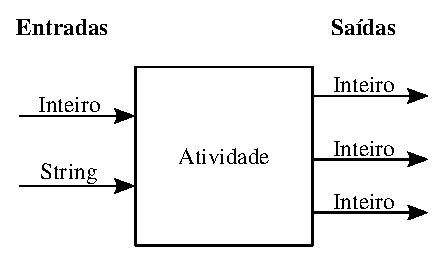
\includegraphics[width=5cm,height=3cm]{./secoes/conceitosFundamentais/pics/img/Atividade.eps}    
	\label{figura_atividade_simples}
	\vspace{0.1cm}
	\source{\varAutorData}
\end{figure}

O segundo tipo de atividade é denominado \emph{Shim}, tem por objetivo adaptar diferentes tipos de dados (como na figura \ref{figura_atividade_shim}\emph{a}). A \emph{atividade} \(1\), da figura \ref{figura_atividade_shim}\emph{a}, tem como saída um \emph{id} do tipo \emph{long} e a \emph{atividade} \(2\), tem como entrada um \emph{id} do tipo inteiro, como consequência ambas são incompatíveis. As atividades do tipo \emph{Shim} efetuam conversões de tipos de dados permitindo a conexão entre atividades incompatíveis como na figura \ref{figura_atividade_shim}\emph{b} \cite{Lin2009}.

\begin{figure}[!htp]
    \centering  
    \caption{Exemplo de atividade do tipo \emph{Shim}}
    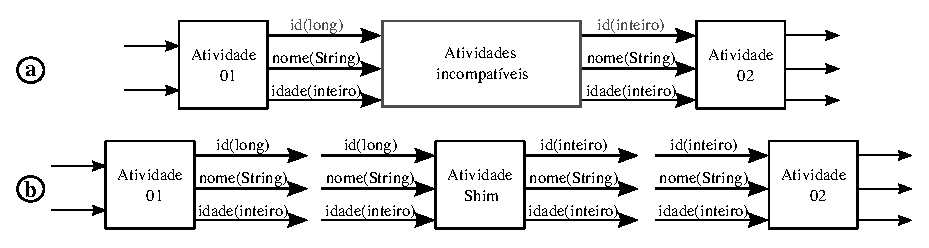
\includegraphics[width=13cm,height=6cm]{./secoes/conceitosFundamentais/pics/img/Shim.eps}    
	\label{figura_atividade_shim}
	\vspace{0.1cm}
	\source{\varAutorData}
\end{figure}

O terceiro tipo é denominado \emph{subworkflow}, que é uma atividade constituída por um \emph{workflow} interno (conjunto de outras atividades), como exibido na figura \ref{figura_atividade_subworkflow} \cite{Medeiros2005}. Nesse caso, o processamento da atividade é efetuado por um \emph{workflow} completo, cujas entradas e saídas devem conter no mínimo as entradas e saídas do \emph{workflow} interno. Há vários tipos de processamentos internos de atividades, os quais variam de acordo com a estrutura do \emph{workflow}. As mais comuns executam um serviço \emph{web} ou código fonte interno, porém no caso de \emph{subworkflows} é comum usar um processamento misto. 

Durante a construção ou execução dos \emph{workflows} (inserção de atividades ou conexão entre as diferentes atividades) alguns SGWCs armazenam as informações relativas à modelagem e execução. Essas informações são conhecidas como proveniência. Segundo \citeonline{Lim2010}, há dois tipos de proveniência: i) \emph{prospective provenance} que modela a especificação de um \emph{workflow}, funcionando como uma abstração/receita do mesmo e que pode ser capturada durante a construção; e ii) \emph{retrospective provenance} que representa as execuções dos \emph{workflows}, quais tarefas foram executadas e quais transformações sobre os dados ocorreram. Esse tipo de proveniência pode ser capturado durante a execução do \emph{workflow}.

\begin{figure}[!htp]
    \centering  
    \caption{Exemplo de atividade do tipo \emph{subworkflow}}
    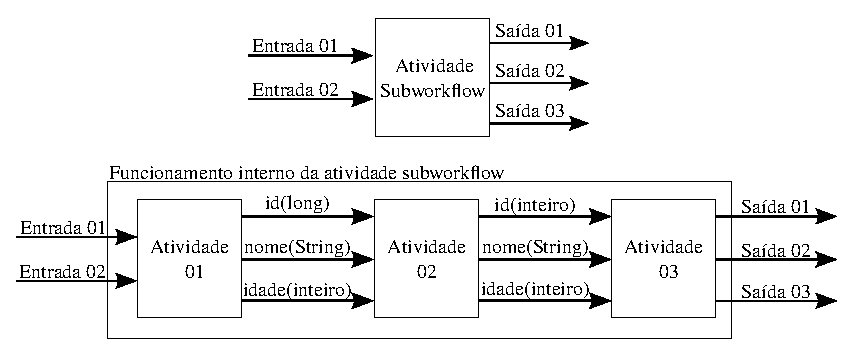
\includegraphics[width=15cm,height=7cm]{./secoes/conceitosFundamentais/pics/img/Subworkflow.eps}    
	\label{figura_atividade_subworkflow}
	\vspace{0.1cm}
	\source{\varAutorData}
\end{figure}

Para auxiliar na construção de \emph{workflows} foram propostas técnicas para compor automaticamente ou recomendar atividades. Na primeira, o usuário passa para o sistema um problema a ser resolvido e o SGWC seleciona e conecta automaticamente as atividades construindo \emph{workflows} para o usuário. Essa técnica é adequada a usuários que não conhecem detalhes específicos do processo e/ou não desejam se envolver nas especificidades de como o \emph{workflow} irá resolver o problema. 

A segunda técnica ocorre durante a construção manual dos \emph{workflows} e o sistema gerenciador sugere ao usuário algumas atividades que podem ser úteis para o \emph{workflow} em construção. 
A técnica de recomendação é indicada para usuários mais experientes que desejam ter participação ativa na construção do \emph{workflow}.
Há três possibilidades muito conhecidas para recomendar atividades. A primeira é baseada em medidas de similaridade e/ou compatibilidade (ver seção \ref{SEC_SISTEMAS_RECOMENDACAO}). A segunda busca atividades em \emph{workflows} ``parecidos'' com o que está sendo desenvolvido. A terceira busca atividades usadas por usuários com perfil semelhante ao do usuário atual. 


\section{Sistemas de recomendação}\label{SEC_SISTEMAS_RECOMENDACAO}
Sistemas de recomendação têm como objetivo recomendar itens que sejam interessantes aos usuários, formalizando: seja \(C\) o conjunto de todos os usuários, \(S\) o conjunto de todos os itens que podem ser recomendados, \(u\) a função de utilidade que metrifica o quanto um item \(s\) é útil para um determinado usuário \(c\),
dada por 
\begin{align}
u : C \times S \rightarrow \mathbb{R}
\end{align}
para cada usuário \(c \in C \) se deseja escolher \(s^{'} \in S \) que maximize a função de utilidade 
\begin{align}
\forall c \in C,  \quad s_{c}^{'} =  \operatorname*{arg\,max}_{s \in S} u(c,s) \label{formalizar_recomendacao}
\end{align}
Em sistemas de recomendação, a função utilidade \(u\) não está definida para todo o espaço {\(C \times S\)}, isso obriga os sistemas de recomendação a extrapolar o espaço conhecido \cite{Adomavicius2005}. Em outras palavras, recomendando itens não que não foram selecionados como \emph{úteis} pelos usuários mas que serão considerados úteis.

Para solucionar esse problema foram propostas diferentes técnicas para recomendar itens, as quais foram organizadas por \citeonline{Paiva2013} em seis classes. A primeira, chamada \emph{filtro baseado em conteúdo}, recomenda itens similares a outros selecionados anteriormente pelo próprio usuário, suas limitações são: i) análise limitada do conteúdo do item que será recomendado, geralmente há falta de descrição semântica do item; ii) superespecialização: o usuário recebe recomendações similares demais às suas escolhas prévias; e iii) novos usuários precisam avaliar um número mínimo de itens antes que o sistema possa recomendar itens para eles.

A segunda, denominada \emph{filtro colaborativo}, recomenda ao usuário itens que já foram selecionados por outros usuários ``similares'' a ele, possuindo como limitações: i) o problema de novos usuários (como identificar com quem eles são similares?); ii) novos itens somente serão recomendados ao passo que forem sendo avaliados por usuários; iii) dados esparsos, alguns poucos usuários costumam avaliar muitos itens e a maioria avalia poucos itens tornando a matriz de utilidade (usuários \(\times\) itens) esparsa, pois o número de avaliações feitas tende a ser muito menor do que o número de sugestões a serem realizadas. Dessa forma, itens raros (que foram avaliados por poucos) dificilmente serão recomendados.

A terceira, denominada \emph{estratégia híbrida}, combina características das técnicas existentes tentando minimizar suas limitações.

Na quarta, conhecida por \emph{filtro baseado na comunidade}, a recomendação é realizada de acordo com a preferência dos colegas ou amigos do usuário ao invés de preferências de desconhecidos. Trata-se de um tipo de especialização do \emph{filtro colaborativo} herdando suas características. Tipicamente, é baseada em informações da rede social (comunidade) do usuário.

A quinta, denominada \emph{demográfica}, utiliza atributos como região, idade e idioma para recomendar. Surgiu para tentar minimizar o problema de esparsidade e é uma especialização do filtro colaborativo considerando que usuários com dados demográficos parecidos podem ser considerados similares.

A sexta, conhecida por \emph{baseada em conhecimento}, recomenda itens de acordo com o domínio de aplicação. A função de similaridade estima quanto a descrição do problema é similar a solução recomendada. Tem como limitação a necessidade de descrições semânticas (usando, por exemplo, ontologias) sobre o domínio, usuário e o problema.

As técnicas de recomendação citadas necessitam de uma métrica de similaridade para determinar o quanto dois itens/usuários/conceitos são próximos. \citeonline{ZhongLi2009} definem uma função de similaridade genérica \(s\) na qual o valor \(s(x,x^{'})\) é alto quando \(x\) e \(x^{'}\) são exemplos parecidos/similares/próximos, caso contrário, possuem um valor baixo. Essa função, de uma forma geral, tem seus valores normalizados entre \([0, 1]\).

De acordo com \citeonline{ZhongLi2009}, distâncias são medidas de dissimilaridade, um caso invertido de similaridade, no qual \(s(x,x^{'})\) é baixo quando \(x\) e \(x^{'}\) são exemplos parecidos ou similares, caso contrário, possuem um valor alto. Uma métrica de distância muito utilizada é a distância Euclidiana \cite{Deza2009}, calculada por
\begin{align}
d(\mathbf{x},\mathbf{y}) = \sqrt{  \sum\limits_{i=1}^{n} (x_{i} - y_{i})^{2} } \label{dist_euclidiana}
\end{align}

Outra métrica conhecida é a distância de Manhattan \cite{Deza2009}, calculada por
\begin{align}
d(\mathbf{x},\mathbf{y}) = \sum\limits_{i=1}^{n} |x_{i} - y_{i}|\label{dist_manhattan}
\end{align}
Uma medida de similaridade muito conhecida é a similaridade da correlação de Pearson \cite{Deza2009}, calculada por
\begin{align}
sim(\mathbf{x},\mathbf{y}) &= \frac{\sum\limits_{i=1}^{n} (x_{i}-\bar{x})(y_{i} - \bar{y})}
{\sqrt{ \left( \sum\limits_{j=1}^{n}(x_{j}-\bar{x}) \right) ^{2} \left( \sum\limits_{j=1}^{n}(y_{j}-\bar{y})\right)^{2}} } \label{similaridade_pearson}
\end{align}
em que \(\bar{y}\) e \(\bar{x}\) representam a média dos dados (\(y\) e \(x\)). Uma distância conhecida para comparar \emph{strings} é a distância de Levenshtein~\cite{Deza2009}, calculada por
\begin{align}
d_{L}(\mathbf{x},\mathbf{y}) = min\{d_{H}(x^{*}, y^{*})\} \label{dist_Levenshtein}
\end{align}
em que \(x^{*}, y^{*}\) são \emph{strings}, \(d_{H}\) é a função que retorna as possibilidades de alteração de \emph{strings} que resultem em duas strings idênticas. A equação \eqref{dist_Levenshtein} representa o número mínimo de alterações necessárias para tornar duas \emph{strings} iguais.

\section{Recomendação em \emph{workflows} científicos}\label{SEC_RECOMENDACAO_WORKFLOW_CIENTIFICO}
A construção de um sistema de recomendação para \emph{workflows} científicos leva em consideração dois aspectos principais. O primeiro, assim como em qualquer sistema de recomendação, é recomendar itens que satisfaçam ao usuário (como descrito na equação \eqref{formalizar_recomendacao}). Já o segundo aspecto está relacionado à resolução de problemas específicos da recomendação de atividades para \emph{workflows} científicos que são: i) restrições de dependência entre entrada e saída de atividades; ii) dependência semântica entre atividades; e iii) ordem das atividades.

A dependência entre entrada e saída de atividades implica que o tipo de dado (inteiro, \emph{string}, \emph{boolean}) das saídas da atividade recém adicionada no \emph{workflow} (anterior à recomendação) devem ser compatíveis com os tipos de dados das entradas da atividade a ser recomendada, que virá a seguir na ordem de execução. Suponha que a atividade \emph{A} tem como saída dois inteiros e uma \emph{string}. Dessa forma, qualquer outra atividade \emph{B} a ser recomendada para completar o \emph{workflow} que contém \emph{A} deve ter como entrada dados compatíveis com estes três tipos (ou com um subconjunto deles), ou será necessária a utilização de uma atividade do tipo \emph{Shim}.

Conectar duas atividades por meio de compatibilidade de entrada e saída ou indiretamente, com uso de atividades \emph{Shim} (como na figura \ref{figura_atividade_shim}) não garante que o \emph{workflow} execute ou que o problema do usuário seja solucionado. Isso ocorre em função da possível incompatibilidade semântica entre atividades como na figura \ref{figura_Incompatibilidade_Semantica}, 
na qual as duas atividades são compatíveis sintaticamente (as entradas e saídas das atividades têm os mesmos tipos de dados), porém enquanto a \emph{string} de saída da atividade \(01\) representa o caminho de um arquivo do sistema operacional, a \emph{string} de saída da atividade \(03\) representa uma conexão com um banco de dados.
\begin{figure}[!hbt]
    \centering  
    \caption{Exemplo de incompatibilidade semântica entre atividades}
    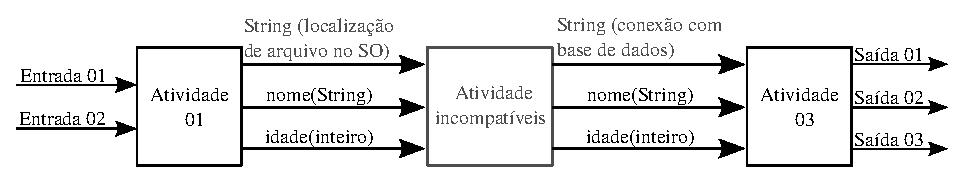
\includegraphics[width=13cm,height=4cm]{./secoes/conceitosFundamentais/pics/img/IncompatibilidadeSemantica.eps}    
	\label{figura_Incompatibilidade_Semantica}
	\vspace{0.1cm}
	\source{\varAutorData}
\end{figure}

Além das dependências é necessário conectar as atividades na ordem correta. Ao contrário de sistemas de recomendação de músicas, os quais podem recomendar itens em qualquer ordem sem afetar o resultado final da recomendação, nessa área a ordem das atividades é relevante. Por exemplo, dadas duas atividades: uma que consulte um banco de dados e outra que atualize a informação consultada pela primeira, a ordem de execução dessas atividades trará diferentes resultados.

Essas características motivam a criação de técnicas específicas para recomendar atividades em \emph{workflows} científicos, como as citadas no capítulo \ref{CAP_CORRELATOS}.

\section{Ontologias}\label{SEC_ONTOLOGIA}
Ontologia é um modelo de representação de conhecimento utilizado para descrever conceitos de um domínio e suas relações, provendo um vocabulário compartilhado para eles. Os conceitos são os substantivos de um determinado domínio de conhecimento e as relações representam as possíveis interações/hierarquias entre esses conceitos~\cite{Umamaheswari2012}.

Os elementos básicos, mas não obrigatórios, de uma ontologia são quatro \cite{ALMEIDA2003} e são exemplificados com o auxílio da figura \ref{figura_ontologia}. O primeiro são os conceitos, que são organizados em uma taxonomia e representam a conceitualização de um domínio, representados pelos retângulos. O segundo são as relações, representadas pelas setas, são as interações entre os conceitos de um determinado domínio. O terceiro são os axiomas que são usados para modelar sentenças. E o último são as instâncias, que representam os elementos específicos, em outras palavras os próprios dados \cite{ALMEIDA2003}. 
\begin{figure}[!hbt]
    \centering   
    \caption{Exemplo de ontologia}
    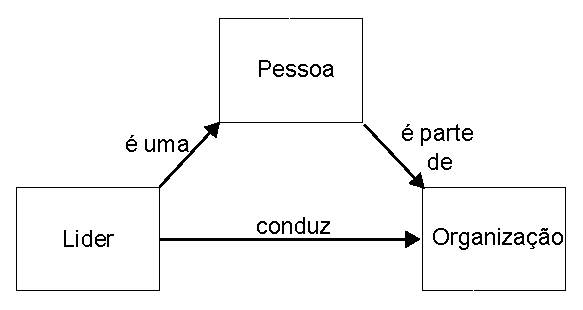
\includegraphics[width=7cm, height=5cm]{./secoes/conceitosFundamentais/pics/img/Ontologia.eps}
    \source{Adaptado de \citeonline{Umamaheswari2012}}
	\label{figura_ontologia}
\end{figure}

Há várias propostas na literatura sobre como classificar ontologias. A tabela \ref{tabela_classificacao_ontologias} apresenta um sumário dessas propostas, organizado por \citeonline{ALMEIDA2003}. Os autores identificaram cinco critérios para classificação de ontologias. O primeiro é baseado em sua função; o segundo considera o grau de formalismo da linguagem usada; o terceiro é em relação a sua aplicação; o quarto é em relação a estrutura (mais genérica ou específica); e o último é em relação ao conteúdo da ontologia.
\bgroup
\def\arraystretch{2}
\begin{table}[htb]
\tiny
\centering
\caption{Possíveis classificações de ontologias}
\begin{tabular}{|l|l|l|}  \hline
\multicolumn{1}{|c}{\textbf{Abordagem}} & \multicolumn{1}{|c|}{\textbf{Classificação}} &  \multicolumn{1}{c|}{\textbf{Descrição}} \\  \hline
%Linha 1
\multirow{3}{*}{\parbox{3cm}{Classificação por \emph{Função} proposta por \citeonline{Mizoguchi1995}}} 			& Domínio       		& Fornecem vocabulário sobre conceitos e seus relacionamentos. \\
				                   						& Tarefa        		& Provê vocabulário sistematizado para diferentes domínios.\\
				                   						& Gerais         		& Vocabulário relacionado a eventos, espaço, casualidade.  \\
\hline 
%Linha 2
\multirow{4}{*}{\parbox{3cm}{Classificação por \emph{Grau de formalismo} proposta por  \citeonline{Uschold96ontologies}}} 	& Informal       		& Linguagem natural  \\ [0.1cm] 
										                & Seminformal        	& Linguagem natural restrita.     			 \\ 
										                & Semiformal         	& Linguagem artificial definida formalmente. \\ 
										                & Formal             	& Semântica formal, teoremas e provas.       \\ 
						                
\hline
%Linha 3
\multirow{3}{*}{\parbox{3cm}{Classificação por \emph{Aplicação} proposta por \citeonline{Jasper99aframework}}} 	& Autoria neutra        & Aplicativo escrito para um sistema e usado em outros.         \\ [0.1cm]
									                    & Especificação        	& Criada para a manutenção e desenvolvimento de sistemas.   \\  
									                    & Acesso comum          & Torna o vocabulário inteligível quando este é ininteligível.\\
\hline
%Linha 4
\multirow{3}{*}{\parbox{2.5cm}{Classificação por \emph{Estrutura} proposta por  \citeonline{haav2001context}}} & Alto nível       & Descrevem conceitos gerais não relacionados ao domínio.         \\ 
	                   						& Domínio          		& Descrevem conceitos gerais relacionados ao domínio. \\ 
	                   						& Tarefa           		& Descrevem atividades com escopo inferior aos conceitos de domínio.  \\ 
\hline  
%Linha 5
\multirow{7}{*}{\parbox{3cm}{Classificação por \emph{Conteúdo} proposta por  \citeonline{vanHeijst1997}}} 			& Terminológica     	    & especificam termos usados para representar um domínio.        \\ 
									                    & Informação   		        & Estruturas de registros de bases de dados.         \\ 
									                    & \parbox{2.5cm}{Modelagem de conhecimento} & Especificam conceitualização do conhecimento.         \\
									                    & Aplicação             	& Definições para modelar o conhecimento uma aplicação   \\
									                    & Domínio             		& Conceitualizações específicas de um domínio.  \\ 
									                    & Genérica             		& Conceitualizações genéricas usadas em vários domínios.  \\
									                    & Representação             & Conceitualismo usados para representação do conhecimento.         \\    \hline
\end{tabular}

\label{tabela_classificacao_ontologias}
\vspace{0.1cm}
\source{Adaptado de \citeonline{ALMEIDA2003}}
\end{table}
\egroup

Para utilizar ontologias em sistemas de recomendação é necessário definir uma métrica de similaridade entre ontologias ou entre conceitos de uma mesma ontologia. Segundo \citeonline{Sanchez2012}, essa métrica pode ser calculada por três principais abordagens: i) contagem por arestas; ii) características da ontologia; e iii) conteúdo da informação. A contagem de arestas utiliza a representação em grafos de ontologias em que cada conceito é representado por um nó e as relações entre os conceitos (por exemplo, relações taxonômicas) são representadas por arestas. Essa abordagem calcula o caminho mínimo de arestas entre dois conceitos. Suas principais limitações são: i) não considerar outros possíveis caminhos ou medidas de similaridade (entre conceitos); e ii) utilizar o mesmo peso para todas as arestas.

A abordagem baseada em características das ontologias utiliza a diferença entre as propriedades em comum dos conceitos e as propriedades para calcular a similaridade. As propriedades citadas são, por exemplo, os sinônimos ou definições textuais que os conceitos contenham (mas não é mandatório que os conceitos das ontologias contenham essas propriedades). As limitações dessa abordagem são exigir que a ontologia tenha propriedades além da taxonomia e a dificuldade de identificar os pesos corretos a serem atribuídos para cada propriedade \cite{Sanchez2012}.

A abordagem baseada em conteúdo da informação presente nas ontologias calcula a similaridade baseada na coocorrência de termos entre duas ontologias. Por exemplo, utilizando a equação 
\begin{align}
IC(x) = - \log_2 P(x) 
\end{align}
que calcula o \(\log_2\) da probabilidade de ocorrência \(P(x)\) e multiplica-o por \(-1\). Sua limitação é que necessita de uma grande e refinada estrutura ontológica/taxonômica para conseguir discriminar diferentes conceitos~\cite{Sanchez2012}.

\section{Recomendação a partir de banco de \emph{workflows}}\label{SEC_RECOMENDACAO_BASE_WORKFLOWS}
Uma estratégia para se recomendar atividades em um \emph{workflow} é a baseada nas suas atividades existentes. Neste tipo de estratégia, com base nas atividades existentes no \emph{workflow} atual (em construção) procura-se por atividades que foram úteis a \emph{workflows} finalizados. Para isso, algum critério de proximidade entre \emph{workflows} ou entre atividades costuma ser utilizado. A seguir algumas abordagens que usam banco de dados de \emph{workflows} são apresentadas.

\subsection{Recomendação a partir da última atividade}
Uma maneira de se recomendar atividades com base num banco de \emph{workflows} é sugerir ao usuário as atividades que costumam ser mais frequentemente utilizadas após a última atividade inserida pelo usuário. Essa estratégia assume que a sequência de atividades costuma ser conservada entre diferentes \emph{workflows}.

\subsection{Recomendação a partir de \emph{itemsets}}\label{AAPRIORI}
Uma das maneiras de recomendar itens é por meio da identificação de \emph{itemsets} frequentes (Conjuntos de itens que ocorrem com frequência no conjunto de dados \cite{HanKamber2011}). Um dos algoritmos mais famosos para este tipo de recomendação é o algoritmo \emph{Apriori} \cite{Agrawal1994}.

Algumas definições essenciais para compreender o algoritmo \emph{Apriori} são; i) \emph{itemsets}; ii) \emph{k-itemset}; iii) regra de associação; iv) suporte; iv) confiança; e v) propriedade \emph{Apriori}. Cada conjunto de itens é denominado \emph{itemset} \cite{HanKamber2011}. Um \emph{itemset} com \(k\) elementos é chamado de \emph{k-itemset}. Uma regra de associação é uma relação entre \emph{itemsets} e tem o formato \(A \rightarrow B\). Cada regra de associação tem um suporte dado por
\begin{align}
sup(A \rightarrow B) =  P(A \cup B)
\end{align}
e uma confiança calculada como
\begin{align}
conf(A \rightarrow B) =  \frac{sup(A \rightarrow B)}{sup(A)}
\end{align}
Uma regra de associação \(r\) é considerada interessante caso \(sup(r) > \alpha\) e \(conf(r) > \beta\). A propriedade \emph{Apriori} diz que para um \emph{itemset} ser considerado frequente todos os \emph{itemsets} contidos nele também devem ser frequentes \cite{HanKamber2011}. Para determinar boas regras de associação deve-se estabelecer dois limiares \(\alpha\) e \(\beta\) para o suporte e a confiança da regra, respectivamente.

O Apriori pesquisa por \emph{itemsets} frequentes, que são aqueles que apresentem um suporte mínimo, em uma base de transações usando uma estratégia de três fases iterativas. 

A primeira é a geração de \emph{itemsets} candidatos de tamanho \(k\) usando os \emph{itemsets} de tamanho \(k-1\), de acordo com a propriedade \emph{Apriori} para aumentar as chances de gerar \emph{itemsets} frequentes devem ser criados apenas \emph{itemsets} que contenham \(k-2\) itens em comum. A segunda fase é a poda, na qual são pesquisados \emph{itemsets} que contenham \emph{subitemsets} não frequentes, os quais são removidos do conjunto de \emph{itemsets} candidatos. A última fase é o cálculo de suporte, na qual cada candidato tem seu suporte calculado varrendo-se a base de dados uma vez, removendo os que contenham suporte menor que o mínimo. 

Um caso especial desse algoritmo é a criação do \emph{itemset} para \(k = 1\), aqueles que contêm apenas um item no conjunto. Dessa forma, não podem ser criados a partir de um conjunto de tamanho inferior como no caso geral descrito anteriormente. Nesse caso são criados todos os possíveis conjuntos unitários. Em seguida, a base de dados é usada para calcular seus suportes. Por fim, são removidos os que não contêm suporte mínimo \cite{HanKamber2011}.
\begin{table}[!htb]
 \caption{Bases de dados de exemplo}
   \begin{subtable}{.5\linewidth}
    	\centering
   		\begin{tabular}{|l|l|} \hline 
   			\textbf{id} & \textbf{Produto} 		\\ \hline 
	   		 1	& Pão                 			\\ \hline 
	   		 2	& Leite            				\\ \hline 
	   		 3  & Açúcar             			\\ \hline
	   		 4  & Papel Higiênico    			\\ \hline
	   		 5  & Manteiga           			\\ \hline
	   		 6  & Fralda             			\\ \hline
	   		 7  & Cerveja            			\\ \hline
	   		 8  & Refrigerante      			\\ \hline
	   		 9  & Iogurte            			\\ \hline
	   		 10 & Suco	         				\\ \hline
   		\end{tabular}
   		\vspace{0.1cm}
   		\caption{Produtos da base de dados}   
   		\label{TABAPRIORI:PRODUTOSMERCADO}		
   \end{subtable}%
   \begin{subtable}{.5\linewidth}
   		\centering
   		\begin{tabular}{|c|l|l|l|l|} \hline 
   		\textbf{TID} & \textbf{Itens comprados}		\\ \hline 
   		101                & \{1, 3, 5\}			\\ \hline 
   		102                & \{2, 1, 3, 7, 5\}	 	\\ \hline
   		103                & \{4, 9, 2, 1\}    		\\ \hline
   		104                & \{5, 2, 1, 3, 9\}   	\\ \hline
   		105                & \{1, 8, 6, 4, 3, 5\}	\\ \hline
   		106                & \{9, 2, 8\}  			\\ \hline
   		\end{tabular}
   		 \caption{Compras efetuadas no supermercado}
   		 \label{TABAPRIORI:ITEMSETS}
   \end{subtable}
\label{TABAPRIORI}
\vspace{0.1cm}
\source{Adaptado de \citeonline{HanKamber2011}}
\end{table}

\section{Recomendação por classificação}\label{SEC_RECOMENDACAO_CLASSIFICACAO}
Segundo \citeonline{HanKamber2011} classificar itens computacionalmente é construir um modelo que permita predizer suas classes discretas. Este modelo é construído em duas etapas: a primeira é o treinamento, no qual o classificador está aprendendo com um conjunto de itens rotulados; a segunda é a fase de testes. Nela, o classificador utiliza as regras aprendidas na fase anterior para classificar dados sem rótulo.

\subsection{Classificação por vizinhos mais próximos}
O algoritmo \emph{K-nearest neighbors} (KNN) \cite{HanKamber2011}, usa cada instância dos dados de teste para localizar seus \emph{\(k\)} vizinhos mais próximos (de acordo com alguma métrica de similaridade ou distância) e atribui para essa instância à classe que contém o maior número de vizinhos \cite{HanKamber2011}. Para exemplificar o funcionamento são utilizados os dados da tabela \ref{TAB_DADOS_EXEMPLO_KNN} como conjunto de treinamento.  
\begin{table}[hbt]
\center
\caption{Exemplo de dados de treino para o KNN}
\label{TAB_DADOS_EXEMPLO_KNN}	
	\begin{tabular}{|l|c|c|l|}
	\hline
		\textbf{alimento} & \textbf{doçura} & \textbf{crocância}  & \textbf{rótulo}   \\ \hline		
			uva 		& \(8\) & \(5\) & fruta  		\\ \hline
			feijão  	& \(3\) & \(7\) & vegetal 		\\ \hline
			castanha	& \(3\) & \(6\) & proteína  	\\ \hline
			laranja 	& \(7\) & \(3\) & fruta  		\\ \hline	
			tomate 		& \(6\) & \(4\) & fruta  		\\ \hline	
	\end{tabular}
	\vspace{0.1cm}
	\source{Adaptado de \citeonline{MachineLearningwithR2013}}
\end{table}

Considerando que os dados da tabela \ref{TAB_DADOS_EXEMPLO_KNN} foram utilizados para treinamento e que o algoritmo recebe uma nova instância (o \emph{tomate}) para ser classificada e que ela possui os atributos: i) doçura \( = 6\); e ii) crocância \( = 4\)). O algoritmo calcula as distâncias entre a instância \emph{tomate} e todos os dados de treinamento, como mostra a figura \ref{FIGURA_KNN}, obtendo
\begin{align}
d(\mbox{uva},\mbox{tomate}) &= \sqrt{(6-8)^{2}+(4-5)^{2}} = 2,2		\\
d(\mbox{feijão},\mbox{tomate}) &= \sqrt{(6-3)^{2}+(4-7)^{2}} = 4,2	\\
d(\mbox{castanha},\mbox{tomate}) &= \sqrt{(6-3)^{2}+(4-6)^{2}} = 3,6	\\
d(\mbox{laranja},\mbox{tomate}) &= \sqrt{(6-7)^{2}+(4-3)^{2}} = 1,4									
\end{align}

Determinar a classe da instância \emph{tomate} depende do número \(k\) de vizinhos escolhidos pelo usuário e pelas distâncias calculadas. Utilizando \(k = 1\), a instância seria classificada como fruta, pois o único vizinho (laranja) pertence a este rótulo. Usando \(k = 3\), a instância terá três vizinhos: i) laranja; ii) uva; e iii) feijão; totalizando duas frutas e um vegetal consequentemente o tomate seria classificado como fruta novamente.
\begin{figure}[hbt]
	\centering
 	  \caption{Exemplo de classificação usando o algoritmo KNN}
		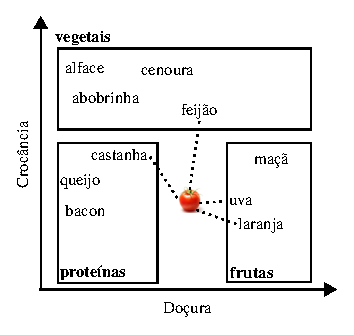
\includegraphics[width=12cm, height=7cm]{./secoes/conceitosFundamentais/pics/img/Tomate.eps}
	\label{FIGURA_KNN}
  \source{Adaptado de \citeonline{MachineLearningwithR2013}}
\end{figure}

A escolha de um número muito alto \(k\) de vizinhos usados para classificar causa uma redução no impacto de ruídos, porém pode enviesar o classificador tornando-o incapaz de identificar alguns padrões significativos. Em contrapartida, utilizar um valor muito baixo, como \(k = 1\), pode tornar o algoritmo suscetível a ruídos.

Uma possível abordagem para encontrar um bom valor de \(k\) é testar o conjunto de dados para diversos valores e comparar as diferentes desempenhos de classificação.

\subsection{Árvores de classificação e regressão - classificador e regressor}\label{SUBSECTION_CART}
Técnicas baseadas em árvores de decisão usam uma estrutura em árvore para tomar decisões. Esta estrutura é constituída por um nó \emph{raiz}, diversos nós de \emph{decisão} e os nós \emph{folha}, como ilustrado na figura \ref{FIGURA_ARVORE_DECISAO}. 

O aprendizado das árvores é feito utilizando o conjunto de treinamento, no qual é selecionado o atributo que maximiza algum critério de divisão (ver equações \eqref{EQ_Ganho_Ganho_Informacao} e \eqref{EQ_Gini_03}) responsável por particionar o conjunto. Este atributo pode se tornar um nó de \emph{decisão}, no caso das instâncias da partição criada por esta divisão contenham rótulos diferentes, ou um nó \emph{folha}, no caso das instâncias da partição criada por esta divisão contenham o mesmo rótulo \cite{HanKamber2011}.
\begin{figure}[hbt]
	\centering
 	  \caption{Estrutura de árvore de decisão}
		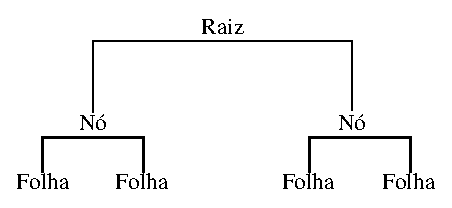
\includegraphics[width=5cm, height=4cm]{./secoes/conceitosFundamentais/pics/img/Arvore.eps}
	\label{FIGURA_ARVORE_DECISAO}
	\vspace{0.1cm}
  \source{Adaptado de \citeonline{Williams2011}}
\end{figure}

O algoritmo CART, proposto por \citeonline{Breiman1984} utiliza uma abordagem \emph{top-down} que constrói a árvore recursivamente selecionando o melhor atributo baseado no índice de \emph{Gini} (ver equação \eqref{EQ_Gini_03}) a cada iteração. O crescimento da árvore termina quando não há mais possibilidade de crescimento, o próximo passo é a poda que constrói \(k\) árvores de decisão nas quais \(T_{1}\) é idêntica a \(T_{0}\) com exceção de um ramo que se transformou em folha e \(T_{k}\) é apenas uma folha. É selecionada a melhor árvore com base no menor erro de classificação \cite{Breiman1984}. 

Alguns critérios de divisão muito utilizados para classificação em árvores de decisão são: i) entropia (conceito da área da Física); e ii) o ganho de informação  (conceito que deriva da teoria da informação). A entropia, mede o grau de incerteza em um conjunto, por exemplo, um conjunto de dados com apenas um valor observado de classe tem entropia igual a zero. Outro conjunto, em que metade dos valores residem em uma classe e a outra metade em outra terá entropia máxima. O cálculo de entropia \cite{HanKamber2011} é descrito pelas seguintes equações
\begin{align}
Entropy(D) &= - \sum\limits_{i=1}^{m}p_{i}\log_{2}(p_{i})\label{EQ_Entropia_Ganho_Informacao} \\
Info_{A}(D) &= \sum\limits_{i=1}^{m}\left(\frac{D_{i}}{D}\right)Entropy(D_{i})\label{EQ_Informacao_AtributoA_Ganho_Informacao}\\
Ganho(A) &= Info(D) - Info_{A}(D)\label{EQ_Ganho_Ganho_Informacao}
\end{align}
sendo \(p_{i}\) a probabilidade da classe \(C_{i}\) no conjunto de dados \(D\), \(m\) é o número de classes, \(D_{i}\) é um subconjunto de \(D\) e a equação \eqref{EQ_Ganho_Ganho_Informacao} calcula o ganho de informação utilizando o atributo \(A\). Esse cálculo é aplicado em todos os atributos e é escolhido o que obtiver maior ganho de informação.

Outro critério que pode ser adotado para a divisão é o índice de \emph{Gini} \cite{HanKamber2011}, que mede a impureza de um conjunto de dados. Representado pelo número de instâncias encontradas na partição que não pertencem a mesma classe, calculada por
\begin{align}
Gini(D) &= 1 - \sum\limits_{i=1}^{m}(p_{i})^{2}\label{EQ_Gini_01} \\
Gini_{A}(D) &= \sum\limits_{i=1}^{m} \left(\frac{D_{i}}{D}\right)Gini(D_{i})\label{EQ_Gini_02} \\
\Delta Gini(A) &= Gini(D) - Gini_{A}(D)\label{EQ_Gini_03}
\end{align}
O atributo escolhido para teste lógico é aquele que maximiza o \(\Delta Gini(A)\).  Em outras palavras, reduz a impureza do conjunto. Esses critérios são usados para particionar os conjuntos de dados de forma recorrente até que se atinja um critério de parada, determinado pelo algoritmo. 

Para tarefas de regressão, o algoritmo tem algumas diferenças. A primeira é usar como métrica de impureza o quadrado da soma residual (SRQ), que, segundo \citeonline{Connor2007}, é calculada por
\begin{align}
\operatorname*{arg\,min}_{x_{j} \leq x_{j}^{R}} \qquad [P_{l}(Var(Y_{l})) + P_{r}(Var(Y_{r}))]
\end{align}
cujo objetivo é minimizar a soma da probabilidade da variância (\(P(Var(Y))\)) dos nós filhos (\(Y_{l}\) nó filho da esquerda e \(Y_{r}\) nó filho da direita) gerados após uma divisão. Outra diferença é que cada nó \emph{folha} será preenchido pela média dos valores das instâncias de treinamento atribuídos na folha. Por fim, supõe-se uma relação linear entre a variável resposta e os preditores. Outros aspectos como construção, poda e treinamento são idênticos a árvores de classificação \cite{Connor2007}.

\subsection{Naive Bayes}
Classificadores baseados em técnicas Bayesianas utilizam os dados de treinamento para calcular a probabilidade observada de cada classe de acordo com suas características. Esses classificadores são melhor aplicados em problemas nos quais a informação de vários atributos pode ser considerada simultaneamente para gerar uma estimativa de probabilidades de saídas.

O algoritmo \emph{Naive Bayes} utiliza a técnica Bayesiana, que é uma aplicação do teorema de Bayes \cite{MachineLearningwithR2013} adaptado para classificação, que assume as seguintes condições ingênuas sobre os dados: i) independência de características; e ii) que todas as características são igualmente importantes. No mundo real, essas condições são falhas, mas ainda assim o algoritmo possui um desempenho satisfatório \cite{HanKamber2011}.

Para explicar o funcionamento da classificação por Naive Bayes será usado um exemplo adaptado de \citeonline{MachineLearningwithR2013}. O objetivo é construir um classificador binário de e-mails com as seguintes classes: i) spam; e ii) não spam. Usando o conjunto de dados de treinamento, cada e-mail é classificado de acordo com a maior probabilidade atribuída pelo classificador (ser spam ou não).

O classificador verifica se o e-mail contém as seguintes palavras \emph{viagra} (\(W_{1}\)), \emph{dinheiro} (\(W_{2}\)), \emph{cancelar assinatura} (\(W_{3}\)) e \emph{comestíveis} (\(W_{4}\)), em seguida,  aplica o teorema de Bayes \cite{MachineLearningwithR2013}. Suponha que o classificador deva rotular a mensagem \(M_{1}\) que contém as palavras: \emph{viagra} e \emph{cancelar assinatura}, para tal, usa-se a seguinte equação
\begin{align}
P(Spam|W_{1} \cap \neg W_{2} \cap \neg W_{3} \cap W_{4}) = \frac{(W_{1} \cap \neg W_{2} \cap \neg W_{3} \cap W_{4})P(Spam)}{(W_{1} \cap \neg W_{2} \cap \neg W_{3} \cap W_{4})} \label{aplicandoBayese-mail}
\end{align}
Os valores usados para o cálculo das probabilidades são obtidos utilizando o conjunto de treinamento (rotulado). A técnica Naive Bayes aplica o conceito de independência de eventos \eqref{independencia} na equação \eqref{aplicandoBayese-mail}
\begin{align}
P(A \cap B) = P(A)P(B) \label{independencia}
\end{align}

Dessa forma, a probabilidade de um e-mail ser classificado como \emph{spam} é dada por
{\footnotesize
\begin{align}
EvSpam &= Spam|W_{1} \cap \neg W_{2} \cap \neg W_{3} \cap W_{4} \label{ProbabilidadeSpamBayesResumo}\\
P(EvSpam) &= \left(\frac{P(W_{1}|Spam) P(\neg W_{2}|Spam) }{P(W_{1}) P(\neg W_{2})}\right)\left(\frac{P(\neg W_{3}|Spam) P(W_{4}|Spam) P(Spam)}{P(\neg W_{3}) P(W_{4})} \right) \label{ProbabilidadeSpamBayes}
\end{align}
}
aplicando-se a fórmula simplificada novamente, obtem-se a probabilidade do e-mail ser classificado como \emph{não spam}, dada por
{\footnotesize
\begin{align}
\overline{EvSpam} &= \overline{Spam}|W_{1} \cap \neg W_{2} \cap \neg W_{3} \cap W_{4} \\
P(\overline{EvSpam}) &= \left( \frac{P(W_{1}|\overline{Spam}) P(\neg W_{2}|\overline{Spam}) }{P(W_{1}) P(\neg W_{2})}\right) \left(\frac{P(\neg W_{3}|\overline{Spam}) P(W_{4}|\overline{Spam}) P(\overline{Spam})}{P(\neg W_{3}) P(W_{4})}\right) \label{ProbabilidadeNaoSpamBayes}
\end{align}
}
Após definir as fórmulas para o cálculo das probabilidades da mensagem, serão utilizados os dados do conjunto de treinamento, exibidos na tabela \ref{tab_verossimilhancasExemploNaiveBayes}, para calcular suas probabilidades e efetuar a classificação.
\bgroup
\def\arraystretch{1.5}
\begin{table}[!htp]
\centering
\caption{Exemplo do cálculo de verossimilhança}
\begin{tabular}{lccccccccc}
\hline
\multicolumn{1}{c}{} & \multicolumn{2}{c}{$\mathbf{W_1}$} & \multicolumn{2}{c}{$\mathbf{W_2}$} & \multicolumn{2}{c}{$\mathbf{W_3}$} & \multicolumn{2}{c}{$\mathbf{W_4}$} \\ \hline
Verossimilhança  &   Sim &   Não   &     Sim       &      Não      &     Sim       &       Sim &      Não      &      Sim         \\  \hline  

Spam   &   \(\frac{4}{20}\) &   \(\frac{16}{20}\)   &     \(\frac{10}{20}\)       &      \(\frac{10}{20}\)      &     \(\frac{0}{20}\)       &       \(\frac{20}{20}\)     &      \(\frac{12}{20}\)      &      \(\frac{8}{20}\)          \\ [4pt]

Não Spam   &   \(\frac{1}{80}\) &   \(\frac{79}{80}\)   &     \(\frac{14}{80}\)       &      \(\frac{66}{80}\)      &     \(\frac{8}{80}\)       &       \(\frac{71}{80}\)     &      \(\frac{23}{80}\)      &      \(\frac{57}{80}\)         \\  [4pt]
 
Total  &   \(\frac{5}{100}\) &   \(\frac{95}{100}\)   &     \(\frac{24}{100}\)       &      \(\frac{76}{100}\)      &     \(\frac{8}{100}\)       &       \(\frac{91}{100}\)     &      \(\frac{35}{100}\)      &      \(\frac{65}{100}\)     \\  \hline
\end{tabular}
\vspace{0.1cm}
	\label{tab_verossimilhancasExemploNaiveBayes}
	\vspace{0.1cm}
	\source{Adaptado de \citeonline{MachineLearningwithR2013}}
\end{table}
\egroup
Usando os dados desta tabela em conjunto com as equações \eqref{ProbabilidadeSpamBayesResumo} até \eqref{ProbabilidadeNaoSpamBayes} obtem-se
\begin{align}
& P(EvSpam) = \left(\frac{4}{20}\right) \left(\frac{10}{20}\right) \left(\frac{20}{20}\right) \left(\frac{12}{20}\right) \left(\frac{20}{100}\right) = 0,012 \\
& P(\overline{EvSpam}) = \left(\frac{1}{80}\right) \left(\frac{66}{80}\right) \left(\frac{71}{80}\right) \left(\frac{23}{80}\right) \left(\frac{80}{100}\right) = 0,002
\end{align}
A probabilidade de ser \emph{spam} é igual a verossimilhança de que a mensagem é \emph{spam} dividida pela probabilidade de ser, ou não \emph{spam}, logo obtem-se
\begin{align}
P(EvSpam) = \frac{0,012}{0,012 + 0,002} = 0,857
\end{align}
De forma análoga para \emph{não spam} tem-se que
\begin{align}
P(\overline{EvSpam}) = \frac{0,002}{0,012 + 0,002} = 0,143 
\end{align}
Pode-se observar que a probabilidade da mensagem \(M_{1}\) ser \emph{spam} é maior que ser \emph{não spam}. Logo será classificada como \emph{spam} pelo algoritmo Naive Bayes.

A teoria da probabilidade Bayesiana é a raiz para o cálculo de verossimilhança de um evento baseado em uma evidência, portanto serão revisados alguns conceitos básicos usados anteriormente. A probabilidade de um evento pode ser obtida pelos dados observados, dividindo o número de ocorrências de um evento pelo número total de dados. Dois eventos são ditos mutuamente exclusivos se eles não ocorrerem ao mesmo tempo. A figura \ref{fig:FIGURA_EVENTOS_MUTUAMENTE_EXCLUSIVOS} apresenta um exemplo de eventos mutuamente exclusivos.
\begin{figure}[!hbt]
\centering
\caption{Tipos de eventos probabilísticos}
\begin{subfigure}{.5\textwidth}
  \centering
  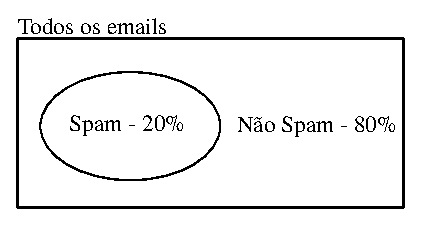
\includegraphics[width=6cm, height=4cm]{./secoes/conceitosFundamentais/pics/img/EventosMutuamenteExclusivos.eps}
  \caption{Eventos mutuamente exclusivos}
  \label{fig:FIGURA_EVENTOS_MUTUAMENTE_EXCLUSIVOS}
\end{subfigure}%
\begin{subfigure}{.5\textwidth}
  \centering
  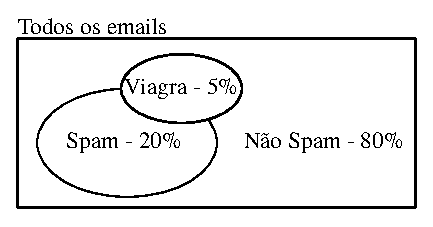
\includegraphics[width=6cm, height=4cm]{./secoes/conceitosFundamentais/pics/img/EventosNaoMutuamenteExclusivos.eps}
  \caption{Eventos não mutuamente exclusivos}
  \label{fig:FIGURA_EVENTOS_NAO_MUTUAMENTE_EXCLUSIVOS}
\end{subfigure}
\label{fig}
\vspace{0.1cm}
 \source{Adaptado de \citeonline{MachineLearningwithR2013}}
\end{figure}
Seja \(P(A)\) a probabilidade de um evento \(A\) ocorrer, e dados dois eventos mutuamente exclusivos \(A\) e \(B\) é válida a seguinte relação
\begin{align}
P(A) = 1 - P(B)
\end{align}
É comum estudar vários eventos não mutuamente exclusivos para a mesma saída, ou seja, eventos que ocorrem em conjunto. Eles permitem que um evento seja utilizado para prever o outro. A figura \ref{fig:FIGURA_EVENTOS_NAO_MUTUAMENTE_EXCLUSIVOS} apresenta um exemplo de eventos não mutuamente exclusivos.

O evento viagra pode (ou não) ser um \emph{spam}, logo ele é um evento conjunto com o evento \emph{spam}, mas nem todo o e-mail com essa palavra é um \emph{spam}. Nesse caso, para prever um evento com base em outro, é necessário calcular a probabilidade da intersecção dos eventos \emph{viagra} e \emph{spam} \(P(Spam \cap Viagra)\) que depende da probabilidade conjunta dos dois eventos (como a probabilidade de um evento está relacionada a outro).

Se todos os eventos forem independentes (não satisfazem a equação \eqref{independencia}) é impossível prever um evento com dados de outro. No caso da não independência, é válida a relação
\begin{align}
P(A|B) =  \frac{P(B|A)P(A)}{P(B)} = \frac{P(A \cap B)}{P(B)} \label{BAYES}
\end{align}

No exemplo da classificação de um e-mail como \emph{spam} ou \emph{não spam}, sem informações adicionais, é possível alegar que há \(20\%\) de chance de ser um \emph{spam}, que é a probabilidade \emph{apriori}.

Agora suponha que foram obtidas mais informações e que a mensagem recebida contenha o termo \emph{Viagra}. A probabilidade desse termo ser utilizado em mensagens anteriores é chamada de \emph{verossimilhança} e a probabilidade do termo aparecer em qualquer mensagem é chamado \emph{verossimilhança marginal}.

Aplicando o teorema de Bayes podemos calcular a probabilidade \emph{posteriori}, usando a equação \eqref{equ_posteriori}, que mede a probabilidade de uma mensagem ser um \emph{spam}. Se a probabilidade for maior que \(50\%\), o e-mail é mais parecido com \emph{spam}.
\begin{align}
P(Spam|Viagra) =  \frac{\overbrace{P(Viagra|Spam)}^{\text{verossimilhança}} \overbrace{P(Spam)}^{\text{probabilidade apriori}}}{\underbrace{P(Viagra)}_{\text{verossimilhança marginal}}} \label{equ_posteriori}
\end{align}
Para calcular os componentes da equação \eqref{equ_posteriori} é necessária uma tabela de frequência, a qual armazena o número de ocorrências do termo \emph{Viagra} nos e-mails classificados como \emph{spam} e como \emph{não spam} (calculada utilizando o conjunto de treinamento), esta tabela será utilizada para construir uma tabela de verossimilhança.
\bgroup
\def\arraystretch{1.5}
\begin{table}[!htb]
	\caption{Matriz de frequência e de verossimilhança}
   \begin{subtable}{.5\linewidth}
    		\centering
    		
    			\begin{tabular}{lccc} \hline
    	
    			Frequência	& \(W_{1}\)		& \( \neg W_{1}\)			& Total   \\ \hline
    			Spam		& \(4\) 		& \(16\)			& \(20\)  \\ 
    			Não Spam	& \(1\) 		& \(79\)			& \(80\)  \\ 
    			Total		& \(5\) 		& \(95\)			& \(100\) \\ \hline
    			
    			\end{tabular}
    			\vspace{0.1cm}
    			\caption{Matriz de frequência}
    		\label{TABVEROSSIMILHANCA:ExemploDeTabela1}
   \end{subtable}%
   \begin{subtable}{.5\linewidth}
   		\centering
   	
   			\begin{tabular}{lccc} \hline
   	
   			Frequência	& \(W_{1}\)			& \( \neg W_{1}\)			& Total   \\ \hline
   			Spam		& \(\frac{4}{20}\) 	& \(\frac{16}{20}\)	& \(20\)  \\ 
   			Não Spam	& \(\frac{1}{80}\) 	& \(\frac{79}{80}\)	& \(80\)  \\ 
   			Total		& \(\frac{5}{100}\) & \(\frac{95}{100}\)& \(100\) \\ \hline
   			
   			\end{tabular}
   			\vspace{0.1cm}
   			\caption{Matriz de verossimilhança}
   		\label{TABVEROSSIMILHANCA:ExemploDeTabela2}
   \end{subtable}
\label{TABVEROSSIMILHANCA}
\vspace{0.1cm}
\source{Adaptado de \citeonline{HanKamber2011}}
\end{table}
\egroup
No exemplo da mensagem \(M_{1}\) foi construída a tabela de frequência \ref{TABVEROSSIMILHANCA:ExemploDeTabela1} que permitiu a construção da tabela de verossimilhança \ref{TABVEROSSIMILHANCA:ExemploDeTabela2}. Esta última, em conjunto da equação \eqref{BAYES}, permite calcular a probabilidade \emph{posteriori} como
\begin{align}
\frac{P(Viagra|Spam)P(Spam)}{P(Viagra)} = \frac{ \left(\frac{4}{20}\right) \left(\frac{20}{100}\right)}{\left(\frac{1}{80}\right)} = 3,2
\end{align}
que é uma probabilidade mais precisa, por considerar a probabilidade condicional do termo \(W_{1}\)(viagra), ao invés da probabilidade baseada em independência.

\subsection{Rede neural - classificador e regressor}
Redes neurais artificiais têm como inspiração o cérebro humano, seus neurônios e suas conexões. A computação tenta reproduzir esse modelo de cérebro como uma relação de entradas e saídas ponderadas, que são conjuntos de nós de processamento. Eles são responsáveis por calcular a soma de entradas ponderadas e repassá-las para a função de ativação, responsável por determinar se um sinal será enviado (ou não) para o neurônio seguinte \cite{Haykin2007}.
\begin{figure}[hbt]
	\centering
 	\caption{Exemplo de neurônio}
	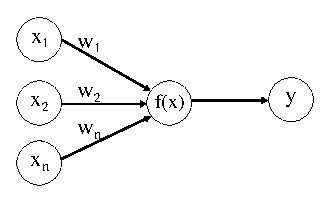
\includegraphics[width=5.5cm,height=3cm]{./secoes/conceitosFundamentais/pics/img/RedeNeural.eps}
	\label{FIGURA_REDE_NEURAL_NEURONIO}
	\vspace{0.1cm}
  	\source{Adaptado de \citeonline{MachineLearningwithR2013}}
\end{figure}

A figura \ref{FIGURA_REDE_NEURAL_NEURONIO} apresenta um neurônio, no qual o vetor \(\mathbf{w}\) contém os pesos sinápticos, o vetor \(\mathbf{x}\) contém os \(n\) sinais de entrada, \(f(x)\) é a função de ativação e \(y\), é o sinal de saída que é calculado por
\begin{align}
y(x) = f \left( \sum\limits_{i=1}^{n} w_{i}x_{i} \right)
\end{align}

Uma rede neural é um conjunto de neurônios conectados em uma determinada \emph{arquitetura}. Ela consiste no número de neurônios por camada, o tipo de conexão entre eles, o fluxo de informação entre neurônios, a função de ativação e o algoritmo de treinamento utilizado. No restante desta seção são detalhados os itens da arquitetura citados.

Analisando a rede neural da figura \ref{FIGURA_REDE_NEURAL_TOPOLOGIA} pode-se constatar que suas camadas são formadas por: i) três neurônios de entrada (representados pela letra \emph{x}), que recebem os dados diretamente da fonte; ii) dois neurônios ocultos (representados por \emph{h}), que recebem dados processados por neurônios e enviam esses dados para outros neurônios; e iii) um neurônio de saída (representado por \emph{y}) que apresenta a saída da rede.
\begin{figure}[hbt]
	\centering
 	  \caption{Topologia de rede neural}
		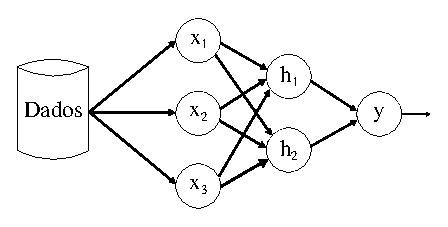
\includegraphics[width=8cm,height=5cm]{./secoes/conceitosFundamentais/pics/img/RedeNeuralTopologia.eps}
	\label{FIGURA_REDE_NEURAL_TOPOLOGIA}
  \source{Adaptado de \citeonline{MachineLearningwithR2013}}
\end{figure}

Neste projeto, serão usadas redes neurais com duas camadas, essa escolha é justificada por \citeonline{Weston2007} que demonstram que o aumento do número de camadas não aumenta a capacidade de generalização e/ou precisão das redes neurais.

O tipo de conexão entre neurônios na figura \ref{FIGURA_REDE_NEURAL_TOPOLOGIA} é denominado \emph{totalmente conectada}, no qual todos os neurônios de uma camada estão conectados com todos os neurônios da camada seguinte. O fluxo de informação é denominado \emph{feedforward} pois os dados trafegam da esquerda para a direita (no sentido das setas pretas) sem retroalimentação.

A função de ativação \(f(x)\), exibida na figura \ref{FIGURA_REDE_NEURAL_NEURONIO}, determina qual tipo de sinal será enviado para o neurônio seguinte. \citeonline{MachineLearningwithR2013} cita as seguintes funções de ativação: a função \emph{degrau} definida por
\begin{align}
f(x) = \begin{cases}
		0 \mbox{ se } x < 0 	 \\
		1 \mbox{ se } x \geq 0	 \label{EQU_FUNCAO_DEGRAU}				
	   \end{cases}
\end{align}
e a função \emph{sigmoide} definida por
\begin{align}
f(x) = \frac{1}{1 + e^{-x}} 	\label{EQU_FUNCAO_SIGMOIDE}
\end{align}

A escolha da função de ativação deve considerar possíveis restrições do algoritmo de treinamento, um exemplo de restrição do algoritmo \emph{backpropagation} é que a função deve ser diferenciável em todos os pontos. Apenas a função \emph{sigmoide} \eqref{EQU_FUNCAO_SIGMOIDE} ,das que foram apresentadas nessa seção, satisfaz essa condição.

O algoritmo de treinamento usado neste projeto, denominado \emph{backpropagation}, possui duas abordagens para treinar os dados: i) \emph{online}; e ii) \emph{batch}. Neste projeto é usada a primeira forma, que atualiza os pesos sinápticos, instância por instância, iterativamente após serem apresentadas a rede neural \cite{Haykin2007}. Para explicar o funcionamento deste algoritmo é necessário compreender como calcular o erro de um neurônio \(j\) na iteração \(n\), como o da figura \ref{FIGURA_REDE_NEURAL_NEURONIO_BACKPROPAGATION} que é calculado por
\begin{align}
e_{j}(n) = d_{j}(n) - y_{j}(n)	\label{EQU_REDE_NEURAL_ERRO_NEURONIO_J}
\end{align}
sendo \(d_{j}(n)\) o valor de saída esperado e \(y_{j}(n)\) o valor de saída obtido. Além desse erro, é necessário calcular o valor de erro total da camada de saída que é calculado por
\begin{align}
\xi(n) = \frac{1}{2} \sum\limits_{j = 1}^{|C|} e_{j}^{2}(n)	\label{EQU_REDE_NEURAL_ERRO_TODOS_OS_NEURONIOS_SAIDA}
\end{align}
sendo \(|C|\) o número de neurônios na camada de saída da rede. O objetivo do treinamento é atualizar o vetor \(\mathbf{w}\) para minimizar a equação \eqref{EQU_REDE_NEURAL_ERRO_TODOS_OS_NEURONIOS_SAIDA}. Essa minimização é realizada pela técnica \emph{descida de gradiente}, a qual começa calculando o vetor de gradiente de cada neurônio. Em seguida, calcula o erro de cada neurônio para as duas possíveis situações: i) para os neurônios de saída (caso simples); e ii) para os neurônios ocultos (caso complexo). Por fim, usa a regra delta \eqref{EQU_REGRA_DELTA} para atualizar o valor \(\mathbf{w}\), esta regra tem como requisitos os cálculos: i) do vetor gradiente; e ii) o erro dos neurônios.
\begin{figure}[hbt]
	\centering
 	  \caption{Exemplo de neurônio de saída para cálculo do \emph{backpropagation}}
		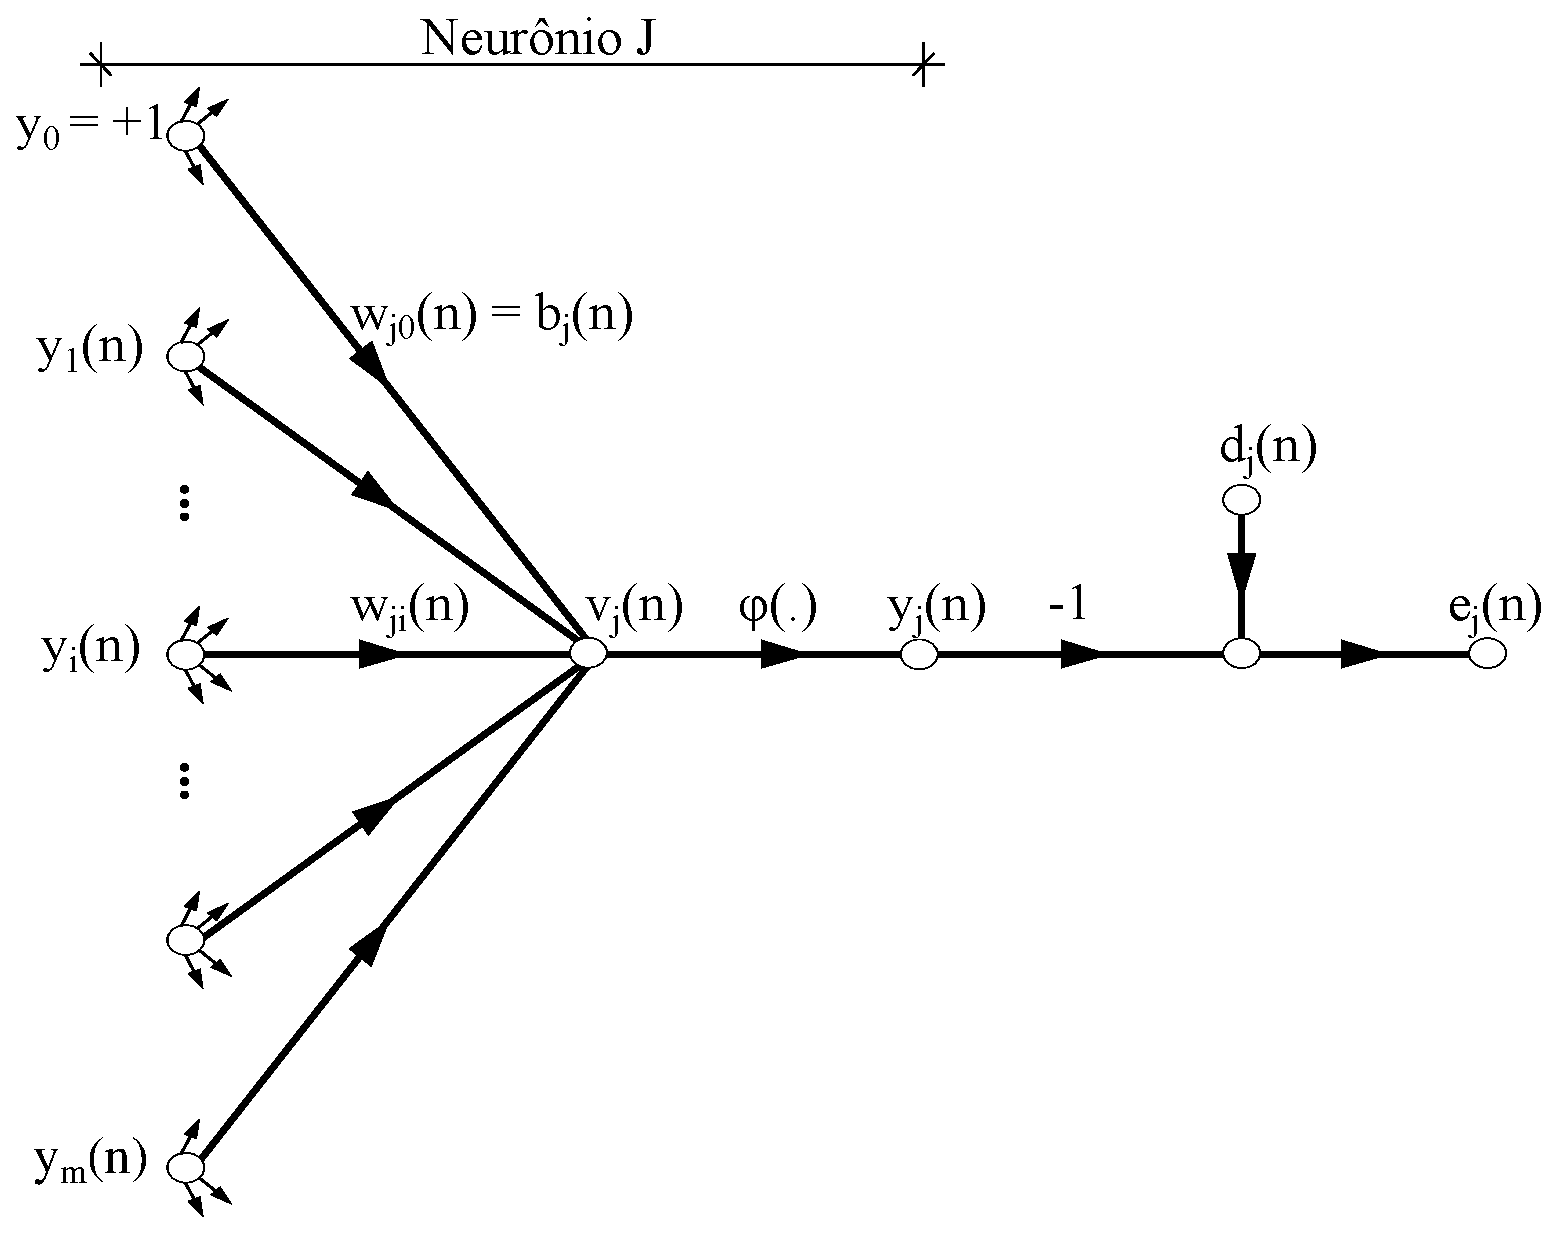
\includegraphics[width=13cm,height=7cm]{./secoes/conceitosFundamentais/pics/img/umNeuronio.eps}
	\label{FIGURA_REDE_NEURAL_NEURONIO_BACKPROPAGATION}
  \source{Adaptado de \citeonline{Haykin2007}}
\end{figure}

A figura \ref{FIGURA_REDE_NEURAL_NEURONIO_BACKPROPAGATION} exibe um neurônio \(j\) sendo alimentado por uma camada de neurônios à esquerda, denominada \(y_{i}\) com \(i = 1, 2, 3 \ldots m\). Esse neurônio tem o valor de entrada da função de ativação \(v_{j}(n)\), que é uma soma ponderada entre as entradas e seus pesos, calculada por
\begin{align}
v_{j}(n) = \left( \sum\limits_{i = 0}^{m} w_{ji}(n)y_{i}(n) \right)  \label{EQU_REDE_NEURAL_SOMA_ATIVACAO_NEURONIO}
\end{align}
sendo \(m\) o número total de neurônios de entrada. O resultado da equação \eqref{EQU_REDE_NEURAL_SOMA_ATIVACAO_NEURONIO} é o parâmetro de entrada para a função de ativação, dessa forma é possível escrever
\begin{align}
y_{j}(n) = \varphi_{j}(v_{j}(n)) \label{EQU_REDE_NEURAL_SAIDA_NEURONIO}
\end{align}

A correção \(\Delta w_{ij}(n)\) aplicada nos pesos sinápticos \(w_{ij}(n)\) é proporcional a derivada parcial do erro total em relação aos pesos sinápticos \(\frac{\partial \xi(n)}{\partial w_{ji}(n)}\) e pode ser escrita, de acordo com a regra da cadeia, como
\begin{align}
\frac{\partial \xi(n)}{\partial w_{ji}(n)} =
\left( \frac{\partial \xi(n)}{\partial e_{j}(n)} 	\right)	\,
\left( \frac{\partial e_{j}(n)}{\partial y_{j}(n)} 	\right) \,
\left( \frac{\partial y_{j}(n)}{\partial v_{j}(n)} 	\right) \,
\left( \frac{\partial v_{j}(n)}{\partial w_{ji}(n)} \right) \label{EQU_REDE_NEURAL_GRADIENTE}
\end{align}
a derivada parcial da equação \eqref{EQU_REDE_NEURAL_GRADIENTE} representa um fator de sensitividade que determina em qual direção no espaço de pesos deve-se pesquisar pelas atualizações de \(w_{ji}(n)\). Cada uma das quatro derivadas parciais do lado direito da equação \eqref{EQU_REDE_NEURAL_GRADIENTE} será solucionada para encontrar o gradiente. Diferenciando os dois lados da equação \eqref{EQU_REDE_NEURAL_ERRO_TODOS_OS_NEURONIOS_SAIDA} em relação à \(e_{j}(n)\) é possível reescrevê-la como
\begin{align}
\frac{\partial \xi(n)}{\partial e_{j}(n)} = e_{j}(n) \label{EQU_REDE_NEURAL_DERIVADA_ERRO_TOTAL_SOBRE_ERRO}
\end{align}
diferenciando os dois lados da equação \eqref{EQU_REDE_NEURAL_ERRO_NEURONIO_J} em relação à \(y_{j}(n)\) é possível reescrevê-la como
\begin{align}
\frac{\partial e_{j}(n)}{\partial y_{j}(n)} = -1 \label{EQU_REDE_NEURAL_DERIVADA_ERRO_NEURONIO_SOBRE_SINAL_SAIDA_NEURONIO}
\end{align}
diferenciando a equação \eqref{EQU_REDE_NEURAL_SAIDA_NEURONIO} em relação à \(v_{j}(n)\) é possível reescrevê-la como
\begin{align}
\frac{\partial y_{j}(n)}{\partial v_{j}(n)} = \varphi^{'}(v_{j}(n)) \label{EQU_REDE_NEURAL_DERIVADA_SAIDA_NEURONIO_SOBRE_SOMA_ATIVACAO_NEURONIO}
\end{align}
diferenciando a equação \eqref{EQU_REDE_NEURAL_SOMA_ATIVACAO_NEURONIO} em relação à \(w_{ji}(n)\) é possível reescrevê-la como
\begin{align}
\frac{\partial v_{j}(n)}{\partial w_{j}(n)} = y_{i}(n) \label{EQU_REDE_NEURAL_DERIVADA_SOMA_ATIVACAO_NEURONIO_SOBRE_PESOS}
\end{align}
%\eqref{EQU_REDE_NEURAL_DERIVADA_ERRO_NEURONIO_SOBRE_SINAL_SAIDA_NEURONIO}, %\eqref{EQU_REDE_NEURAL_DERIVADA_SAIDA_NEURONIO_SOBRE_SOMA_ATIVACAO_NEURONIO}, 
substituindo as equações \eqref{EQU_REDE_NEURAL_DERIVADA_ERRO_TOTAL_SOBRE_ERRO} até \eqref{EQU_REDE_NEURAL_DERIVADA_SOMA_ATIVACAO_NEURONIO_SOBRE_PESOS} na equação \eqref{EQU_REDE_NEURAL_GRADIENTE} pode-se reescrever o erro em função dos pesos da rede como
\begin{align}
\frac{\partial \xi(n)}{\partial w_{ji}(n)} =
-e_{j}(n)\varphi^{'}(v_{j}(n))y_{i}(n)
\label{EQU_REDE_NEURAL_GRADIENTE_VALORES_SUBSTITUIDOS}
\end{align}
a correção \(\Delta w_{ji}(n)\) que será aplicada nos pesos \(w_{ji}(n)\) é definida pela regra delta como
\begin{align}
\Delta w_{ji}(n) = - \eta \left( \frac{\partial \xi(n)}{\partial w_{ji}(n)} \right) 
\label{EQU_REDE_NEURAL_ATUALIZACAO_PESOS}
\end{align}
sendo \(\eta\) a taxa de aprendizado. Substituindo a equação \eqref{EQU_REDE_NEURAL_GRADIENTE_VALORES_SUBSTITUIDOS} na equação \eqref{EQU_REDE_NEURAL_ATUALIZACAO_PESOS} define-se a regra delta como
\begin{align}
\Delta w_{ji}(n) = \eta \delta_{j}(n)y_{i}(n) 
\label{EQU_REDE_NEURAL_ATUALIZACAO_PESOS_COM_GRADIENTE_LOCAL}
\end{align}
na qual o gradiente local \(\delta_{j}(n)\) é definido por
\begin{align}
\nonumber \delta_{j}(n) &= \frac{\partial \xi(n)}{\partial v_{j}(n)} \Leftrightarrow \\ 
 	      \delta_{j}(n) &= \left( \frac{\partial \xi(n)}{\partial e_{j}(n)} \right) \, \left( \frac{\partial e_{j}(n)}{\partial y_{j}(n)} \right) \, \left( \frac{\partial y_{j}(n)}{\partial v_{j}(n)} \right) \Leftrightarrow \label{EQU_REDE_NEURAL_GRADIENTE_LOCAL_ATUALIZACOES}\\
	      \delta_{j}(n) &= e_{j}(n)\varphi^{'}(v_{j}(n))
\label{EQU_REDE_NEURAL_GRADIENTE_LOCAL}
\end{align}

De acordo com a equação \eqref{EQU_REDE_NEURAL_GRADIENTE_LOCAL} o gradiente local \(\delta_{j}(n)\) para o neurônio de saída \(j\) é o produto do sinal de erro da saída \(e_{j}(n)\) para aquele neurônio e o derivativo \(\varphi^{'}(v_{j}(n))\) da função de ativação \cite{Haykin2007}.

A posição do neurônio na arquitetura da rede influência o cálculo do gradiente local. Dessa forma, apresenta papel fundamental para o cálculo do erro. Se for um neurônio de saída pode-se utilizar a equação \eqref{EQU_REDE_NEURAL_ERRO_NEURONIO_J} para determinar \(e_{j}(n)\) que será utilizado para calcular o gradiente local com a equação \eqref{EQU_REDE_NEURAL_GRADIENTE_LOCAL}.
\begin{figure}[hbt]
	\centering
 	  \caption{Exemplo de neurônio oculto para cálculo do \emph{backpropagation}}
		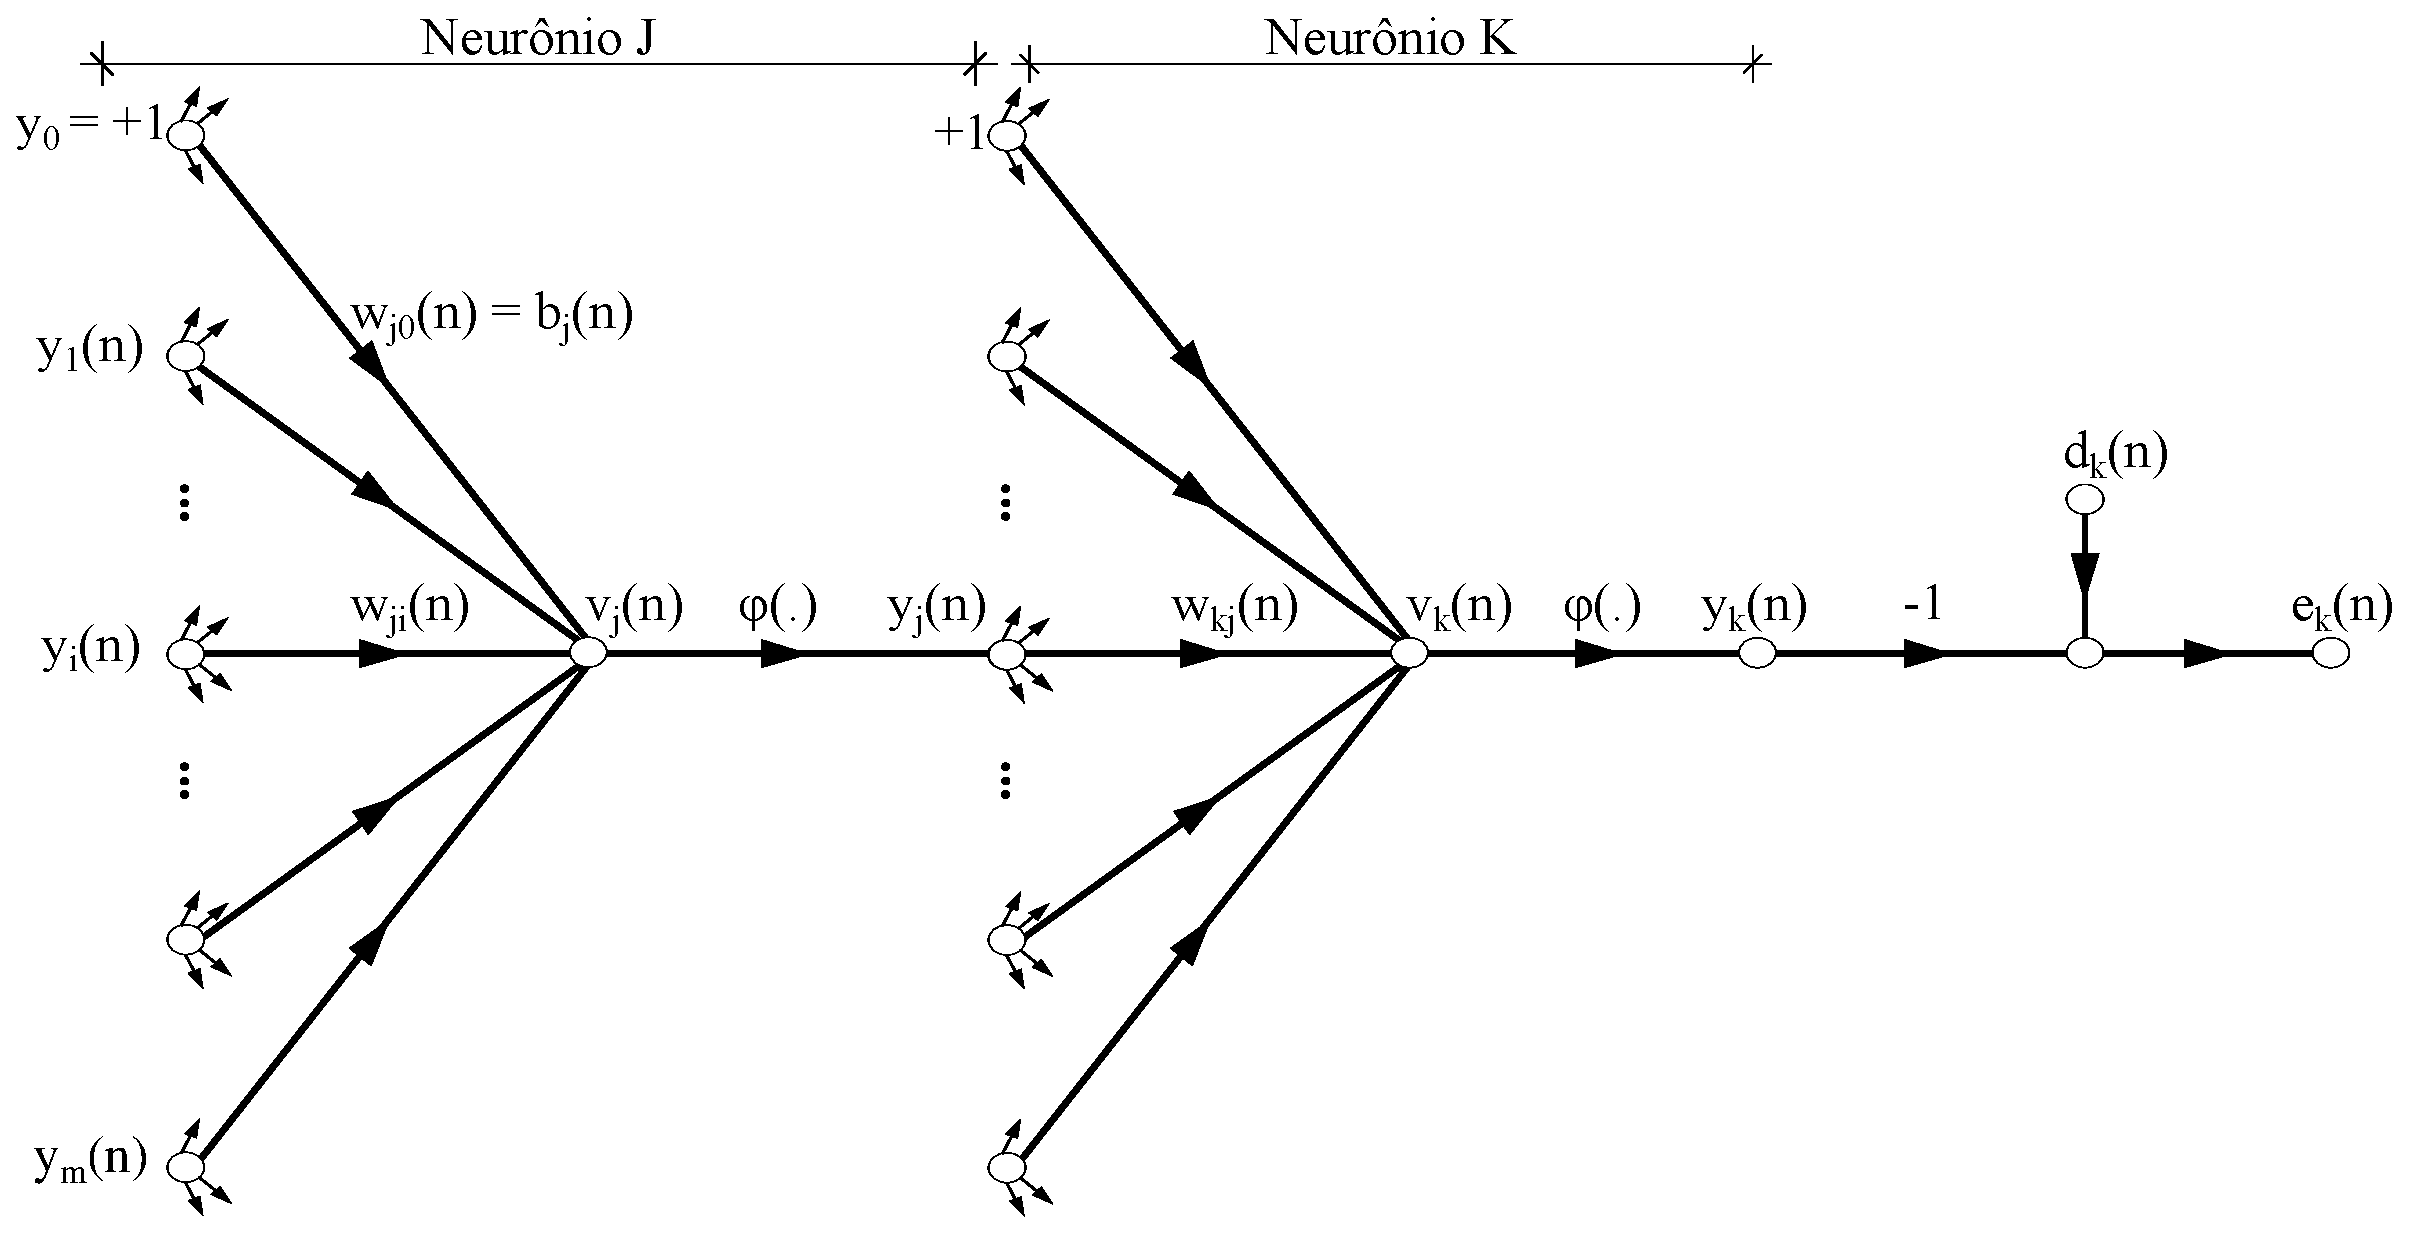
\includegraphics[width=13cm,height=7cm]{./secoes/conceitosFundamentais/pics/img/doisNeuronios.eps}
	\label{FIGURA_REDE_NEURAL_NEURONIOS_BACKPROPAGATION}
  \source{Adaptado de \citeonline{Haykin2007}}
\end{figure}

Se o neurônio estiver localizado em uma camada oculta, não possui erro associado diretamente. Assim, é necessário retropropagar o erro recursivamente pelos neurônios que estão conectados \cite{Haykin2007}. Um exemplo de neurônio oculto pode ser visto na arquitetura da figura \ref{FIGURA_REDE_NEURAL_NEURONIOS_BACKPROPAGATION} em que o gradiente local do neurônio oculto \(j\), de acordo com a equação \eqref{EQU_REDE_NEURAL_GRADIENTE_LOCAL}, é dado por
\begin{align}
\delta_{j}(n) &= - \left( \frac{\partial \xi(n)}{\partial y_{j}(n)} \right) \, \left( \frac{\partial y_{j}(n)}{\partial v_{j}(n)} \right) \Leftrightarrow \label{EQU_REDE_NEURAL_GRADIENTE_LOCAL_CASO2}\\
\delta_{j}(n) &= - \left( \frac{\partial \xi(n)}{\partial y_{j}(n)} \right) \, \varphi^{'}(v_{j}(n))
\end{align}
o erro do neurônio \(j\), exibido pela figura \ref{FIGURA_REDE_NEURAL_NEURONIOS_BACKPROPAGATION}, é dado por
\begin{align}
\xi(n) = \frac{1}{2} \sum\limits_{k = 1}^{|C|} e_{k}^{2}(n) \label{EQU_REDE_NEURAL_ERRO_NEURONIO_OCULTO}
\end{align}
em que \(k\) é um neurônio de saída, diferenciando a equação \eqref{EQU_REDE_NEURAL_ERRO_NEURONIO_OCULTO} em relação à \(y_{j}(n)\) tem-se que
\begin{align}
\frac{\partial \xi(n)}{\partial y_{j}(n)} =  \left( \sum\limits_{k = 1}^{|C|} \frac{\partial e_{k}(n)}{\partial y_{j}(n)} \right)  \label{EQU_REDE_NEURAL_ERRO_NEURONIO_OCULTO_DERIVADA_SAIDA}
\end{align}
usando a regra da cadeia na equação \eqref{EQU_REDE_NEURAL_ERRO_NEURONIO_OCULTO_DERIVADA_SAIDA} pode-se escrevê-la como
\begin{align}
\frac{\partial \xi(n)}{\partial y_{j}(n)} = \sum\limits_{k = 1}^{|C|} \left[ e_{k}(n) \left( \frac{\partial e_{k}(n)}{\partial v_{k}(n)} \right) \left( \frac{\partial v_{k}(n)}{\partial y_{j}(n)} \right) \right]  \label{EQU_REDE_NEURAL_ERRO_NEURONIO_OCULTO_DERIVADA_SAIDA_REGRA_CADEIA}
\end{align}
da figura \ref{FIGURA_REDE_NEURAL_NEURONIOS_BACKPROPAGATION} percebe-se que o erro é dado por
\begin{align}
e_{k}(n) &= d_{k}(n) - y_{k}(n) \Leftrightarrow \\
e_{k}(n) &= d_{k}(n) - \varphi(v_{k}(n))
\end{align}
então é possível reescrever o derivativo da equação \eqref{EQU_REDE_NEURAL_ERRO_NEURONIO_OCULTO_DERIVADA_SAIDA_REGRA_CADEIA} como
\begin{align}
\frac{\partial e_{k}(n)}{\partial v_{k}(n)} &= -\varphi^{'}(v_{k}(n))	\label{EQU_REDE_NEURAL_DERIVATIVO_ERRO_SOBRE_SOMATORIO}	   
\end{align}
a soma ponderada do neurônio \(k\), proposto na figura \ref{FIGURA_REDE_NEURAL_NEURONIOS_BACKPROPAGATION}, é dada por
\begin{align}
v_{k}(n) = \sum\limits_{j = 0}^{m} \left( w_{kj}(n)y_{j}(n) \right)  \label{EQU_REDE_NEURAL_SOMA_PESO_ENTRADA}
\end{align}
sendo \(m\) o número total de entradas (excluindo bias) aplicados no neurônio \(k\), o peso sináptico \(w_{k0}\) é igual ao bias \(b_{k}(n)\) aplicado no neurônio \(k\). Diferenciando a equação \eqref{EQU_REDE_NEURAL_SOMA_PESO_ENTRADA} em relação a \(y_{j}(n)\) é obtido
\begin{align}
\frac{\partial v_{k}(n)}{\partial y_{j}(n)} = w_{kj}(n) \label{EQU_REDE_NEURAL_DERIVATIVO_SOMA_SOBRE_ERRO}
\end{align}
Utilizando as equações \eqref{EQU_REDE_NEURAL_DERIVATIVO_ERRO_SOBRE_SOMATORIO} até \eqref{EQU_REDE_NEURAL_DERIVATIVO_SOMA_SOBRE_ERRO} na equação \eqref{EQU_REDE_NEURAL_ERRO_NEURONIO_OCULTO_DERIVADA_SAIDA_REGRA_CADEIA}, é obtido o seguinte derivativo
\begin{align}
\frac{\partial \xi(n)}{\partial y_{j}(n)} &= -\sum\limits_{k = 1}^{|C|} \left( e_{k}(n)\varphi{'}(v_{k}(n))w_{kj}(n) \right) \Leftrightarrow \\
\frac{\partial \xi(n)}{\partial y_{j}(n)} &= -\sum\limits_{k = 1}^{|C|}\delta_{k}(n)w_{kj}(n) \label{EQU_REDE_NEURAL_ERRO_NEURONIO_SOBRE_SAIDA}
\end{align}

Na segunda linha, é utilizada a definição de gradiente local da equação \eqref{EQU_REDE_NEURAL_GRADIENTE_LOCAL_ATUALIZACOES} trocando o neurônio \(j\) por \(k\). Usando a equação \eqref{EQU_REDE_NEURAL_ERRO_NEURONIO_SOBRE_SAIDA} na equação \eqref{EQU_REDE_NEURAL_GRADIENTE_LOCAL_CASO2} obtem-se a fórmula do gradiente local como
\begin{align}
\delta_{j}(n) = \varphi^{'}(v_{j}(n)) \sum\limits_{k = 1}^{|C|}\delta_{k}(n)w_{kj}(n)
\end{align}

O gradiente local \(\delta_{j}(n)\) exige o cálculo do erro de todos os neurônios da camada seguinte e os pesos sinápticos dessas conexões, dessa forma pode-se escrever a regra delta como
\begin{align}
\Delta w_{ji}(n) = \eta \delta_{j}(n)y_{i}(n) \label{EQU_REGRA_DELTA}
\end{align}
que será usada para atualizar os pesos do vetor \(\mathbf{w}\) no decorrer do treinamento. A técnica de rede neural será usada como classificador e regressor neste projeto. No primeiro caso são usadas as saídas da rede neural para atribuir classes as instâncias. No segundo caso são usados os pesos da rede neural treinada para predizer valores numéricos.

\subsection{SVM Binário} \label{SEC_CONCEITOS_FUNDAMENTAIS_SVM_CLASSIFICACAO}
Suport Vector Machines (SVM) é uma técnica que pode ser usada para classificar dados usando um hiperplano separador. O objetivo do SVM é escolher a posição do hiperplano tal que permita formar partições homogêneas de dados em ambos os lados da superfície de decisão. Considerando dados futuros, a melhor escolha é aquela que maximize a margem entre os dados e o hiperplano separador, nesse caso denominado \emph{hiperplano ótimo} \cite{MachineLearningwithR2013}. 

No decorrer desta seção será detalhada a técnica de SVM, iniciando pelo caso de dados linearmente separáveis, seguida pelo uso das margens flexíveis e finalizando com a generalização com uso do \emph{kernel trick}. As explicações desta seção são baseadas nas obras de \citeonline{Haykin2007}, \citeonline{LIMA2004}, \citeonline{Fletcher1987}, \citeonline{Stewart2013}, \citeonline{Burges1998}, \citeonline{Cristianini1999} e \citeonline{Chang2011}. 

Dado um conjunto de dados linearmente separáveis como
\begin{align}
(\{x_{1}, d_{1}\}), (\{x_{2}, d_{2}\}), \ldots (\{x_{N}, d_{N}\}) \text{ com } \mathbf{x} \in R^{n} \text{ e } d_{i} \in \{+1, -1\}
\end{align}
no qual o vetor \(\mathbf{x}\) representa os dados e o vetor \(\mathbf{d}\) representa as classes. Um hiperplano separador para estes dados é definido pela seguinte equação
\begin{align}
\mathbf{w}^{T}\mathbf{x} + b = 0 		\label{EQU_SVM_HIPERPLANO_DECISAO}
\end{align}
sendo \(\mathbf{x}\) o vetor de entradas, \(\mathbf{w}^{T}\) um vetor de pesos transposto e \(b\) um bias. Este hiperplano, para dados linearmente separáveis, acarreta nas seguintes restrições
\begin{align}
\mathbf{w}^{T}\mathbf{x} + b &\geq 0  	\qquad \textrm{ para } d_{i} = +1 \label{restricaoSVM01} \\
\mathbf{w}^{T}\mathbf{x} + b &< 0		\qquad \textrm{ para } d_{i} = -1 \label{restricaoSVM02}
\end{align}
dados \(\mathbf{w}\) e \(b\), o espaço que separa o hiperplano \eqref{EQU_SVM_HIPERPLANO_DECISAO} e os dados mais próximos é denominado margem de separação (\(\rho\)), a qual pode ser vista na figura \ref{FIGURA_SVM_Vetores_Suporte}. O objetivo do SVM é maximizar essa margem. O hiperplano com margem máxima é conhecido por \emph{hiperplano ótimo}. Tem sua equação definida como
\begin{align}
\mathbf{w_{0}}^{T}\mathbf{x} + b_{0} = 0 								\label{EQU_SVM_HIPERPLANO_OTIMO}
\end{align}
o par de valores ótimos, \(\mathbf{w_{0}}\) e \(b_{0}\), devem satisfazer as seguintes restrições
\begin{align}
\mathbf{w_{0}}^{T}\mathbf{x} + b_{0} &\geq +1  	\qquad \textrm{ para } d_{i} = +1 \label{restricaoSVM010} \\
\mathbf{w_{0}}^{T}\mathbf{x} + b_{0} &< -1		\qquad \textrm{ para } d_{i} = -1 \label{restricaoSVM020}
\end{align}
para garantir que a solução seja única, mesmo reescalando valores de \(\mathbf{w_{0}}\) e \(b_{0}\), pois a equação \eqref{EQU_SVM_HIPERPLANO_OTIMO} permanecerá inalterada \cite{LIMA2004}. Os pontos que satisfazem o sinal de igualdade das condições \eqref{restricaoSVM010} e \eqref{restricaoSVM020} (que são os pontos mais próximos do hiperplano ótimo) são conhecidos por vetores de suporte, que são os pontos destacados na figura \ref{FIGURA_SVM_Vetores_Suporte}. Com essas novas restrições, é possível definir a função discriminante como
\begin{align}
g(x) = \mathbf{w_{0}}^{T}\mathbf{x} + b_{0} 							\label{EQU_SVM_FUNCAO_DISCRIMINANTE}
\end{align}
utilizando a função discriminante é possível definir a margem máxima como uma distância entre: i) hiperplano; e ii) ponto. Pois, para um dado vetor de suporte \(\mathbf{x^{s}}\), para o qual \(d^{s} = +1\), tem-se que
\begin{align}
g(\mathbf{x^{s}}) = \mathbf{w^{T}_{0}}\mathbf{x} + b_{0} = \pm 1 \qquad \textrm{ para } d_{i} = \pm 1
\end{align}
dessa forma é possível escrever a distância entre os vetores de suporte e o hiperplano como
\begin{align}
r = \frac{g(\mathbf{x^{s}})}{||\mathbf{w_{0}}||} = 	\begin{cases} \label{equ_distancia_margem}
														\frac{1}{||\mathbf{w_{0}}||}  \textrm{ para } d^{s} = +1 \\
														\frac{-1}{||\mathbf{w_{0}}||} \textrm{ para } d^{s} = -1
													\end{cases}
\end{align}
usando a equação \eqref{equ_distancia_margem} é possível definir a margem ótima como a distância entre os vetores de suporte da classe \(1\) ao hiperplano ótimo acrescido da distância entre os vetores de suporte da classe \(2\) ao hiperplano ótimo obtendo
\begin{align}
\rho = 2r = \frac{2}{||\mathbf{w_{0}}||} \label{EQU_SVM_MARGEM_MINIMIZAR}
\end{align}
Portanto, para encontrar a margem máxima, \(\rho\) na figura \ref{FIGURA_SVM_Vetores_Suporte}, é necessário maximizar a norma Euclidiana do vetor de pesos definido pela equação \eqref{EQU_SVM_MARGEM_MINIMIZAR} ou de forma equivalente minimizar \(w\) tal que
\begin{align}  
\Phi(w) = \frac{1}{2}\mathbf{w}^{T}\mathbf{w} \label{EQU_SVM_MARGEM_EQUIVALENTE_MAXIMIZAR}
\end{align}
que é um problema de otimização quadrática convexa \cite{LIMA2004} e o fator \(\frac{1}{2}\) foi acrescentado para facilitar as derivações. Esse tipo de problema pode ser solucionado em três etapas. A primeira é construir o lagrangiano, a segunda é derivar as condições de otimização e a terceira é solucionar o problema no espaço dual dos multiplicadores de Lagrange \cite{Haykin2007}.
\begin{figure}[hbt]
  \centering
  \caption{Vetores de suporte e margem do SVM}
  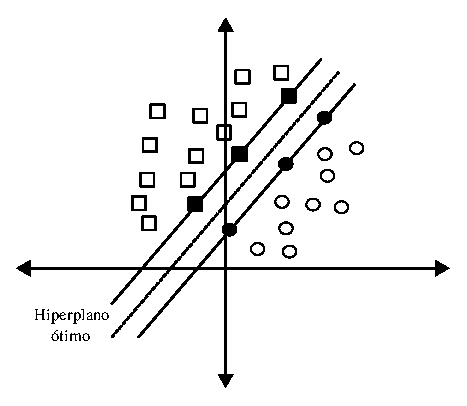
\includegraphics[width=8cm,height=6cm]{./secoes/conceitosFundamentais/pics/img/VetoresDeSuporteSVM.eps}
  \label{FIGURA_SVM_Vetores_Suporte}
  \vspace{0.1cm}
  \source{Adaptado de \citeonline{Haykin2007}}
\end{figure}
\noindent
Para solucionar esse problema de otimização quadrática é utilizada a técnica de multiplicadores de Lagrange \cite{Stewart2013}. Para tal, as restrições \eqref{restricaoSVM010} e \eqref{restricaoSVM020} foram combinadas em apenas uma restrição equivalente
\begin{align}
d_{i}(\mathbf{w}^{T}\mathbf{x} + b )  \geq 1  \qquad \textrm{ para } i = 1, 2, 3, \ldots, N \label{EQU_SVM_RESTRICAO_CONJUNTA}
\end{align}
o que permite escrever o seguinte Lagrangiano
\begin{align}
J(\mathbf{w}, b, \alpha) = \frac{1}{2}\mathbf{w}^{T}\mathbf{w} - \sum\limits_{i=1}^{N} \left\{ \alpha_{i}[d_{i}(\mathbf{w}^{T}\mathbf{x} + b) - 1] \right\} \label{EQU_SVM_LAGRANGIANO_PRIMAL}
\end{align}
no qual o primeiro termo é a função a ser minimizada e o segundo é a restrição reforçada pelos multiplicadores de Lagrange \(\mathbf{\alpha}\). A solução da equação \eqref{EQU_SVM_LAGRANGIANO_PRIMAL} é dada pelo ponto de sela do Lagrangiano (ver figura \ref{FIGURA_SVM_PONTO_DE_SELA}) que deve ser minimizado em relação a \(\mathbf{w}\) e \(b\), isto requer duas condições
\begin{align}
 \frac{\partial J(\mathbf{w}, b, \alpha)}{\partial \mathbf{w}} = 0	\label{EQU_SVM_PONTO_SELA_W}\\
 \frac{\partial J(\mathbf{w}, b, \alpha)}{\partial b} = 0  	\label{EQU_SVM_PONTO_SELA_B}
\end{align}
aplicando a condição \eqref{EQU_SVM_PONTO_SELA_W} na equação \eqref{EQU_SVM_LAGRANGIANO_PRIMAL} obtem-se 
\begin{align}
\mathbf{w} = \sum\limits_{i = 1}^{N} \left( \alpha_{i}d_{i}\mathbf{x_{i}} \right) \label{EQU_SVM_PONTO_SELA_W_RESTRICAO_OBTIDA}
\end{align}
aplicando a condição \eqref{EQU_SVM_PONTO_SELA_B} na equação \eqref{EQU_SVM_LAGRANGIANO_PRIMAL} obtem-se 
\begin{align}
\sum\limits_{i=1}^{N} \left( \alpha_{i}d_{i} \right) = 0 \label{EQU_SVM_PONTO_SELA_B_RESTRICAO_OBTIDA}
\end{align}
\begin{figure}[hbt]
  \centering
  \caption{Ponto de sela do Lagrangiano}
  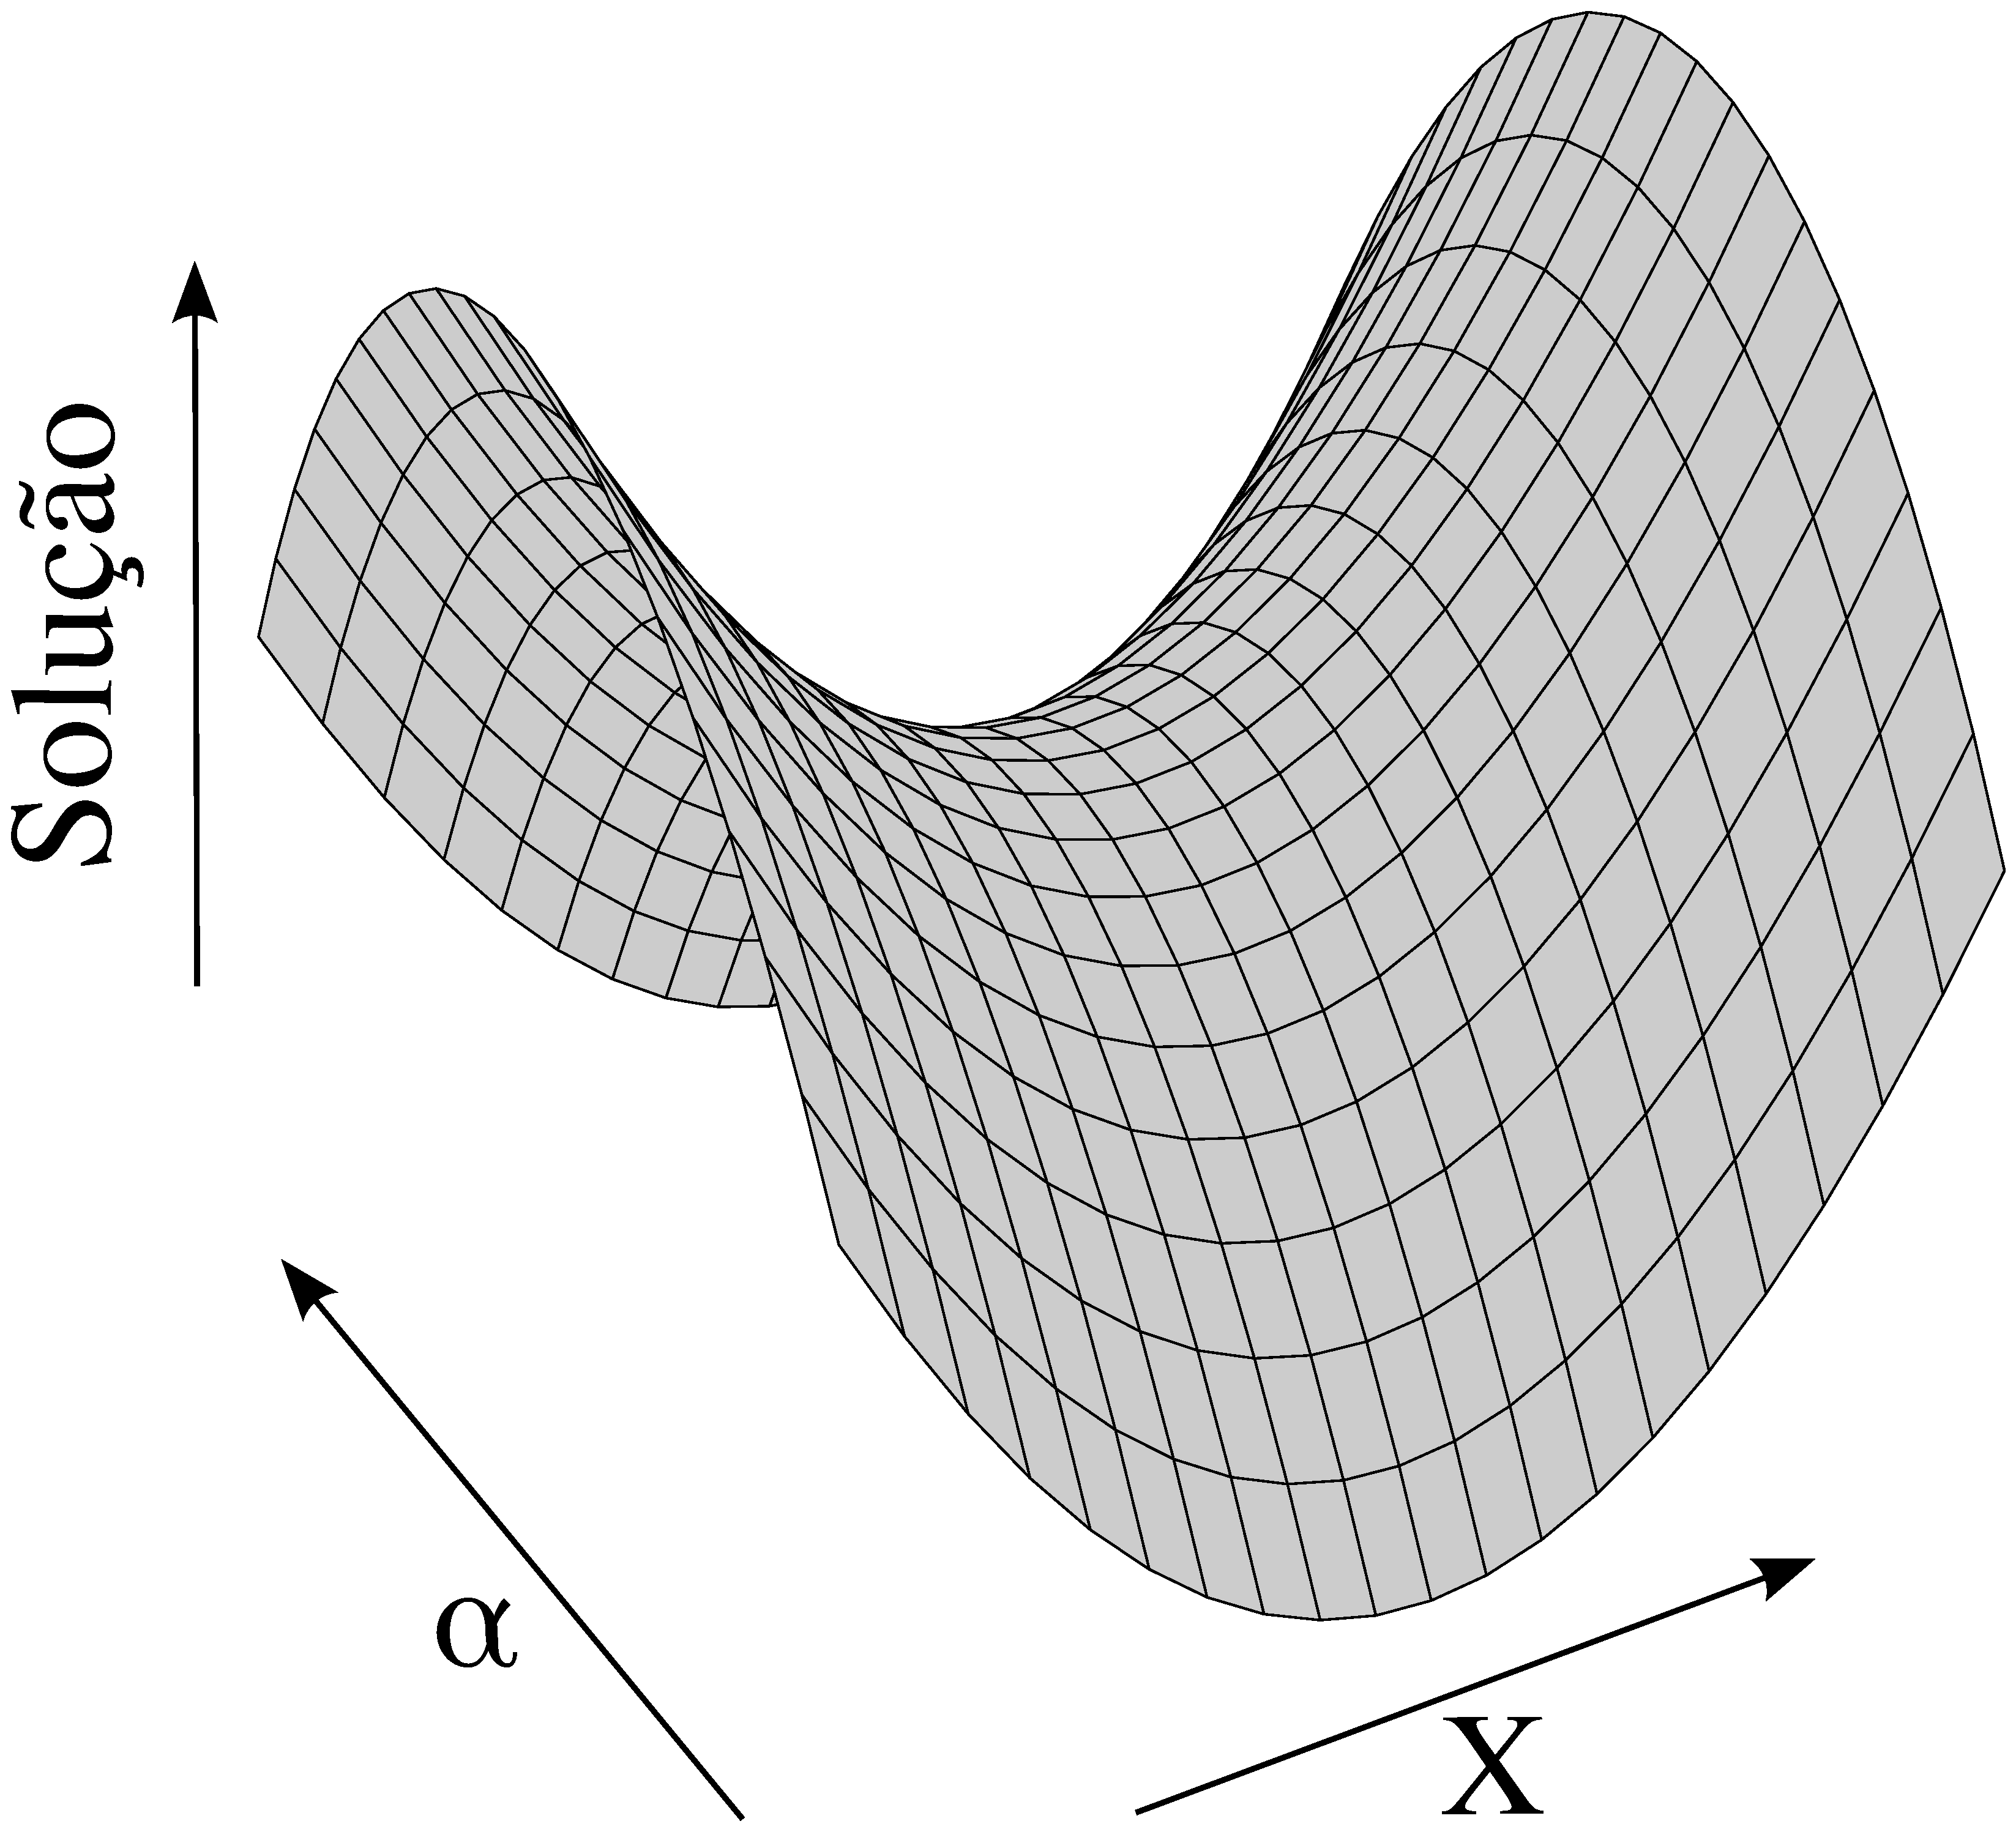
\includegraphics[width=8cm,height=6cm]{./secoes/conceitosFundamentais/pics/img/Rplot.eps}
  \label{FIGURA_SVM_PONTO_DE_SELA}
  \vspace{0.1cm}
  \source{Adaptado de \citeonline{Haykin2007}}
\end{figure}
\noindent
Segundo \citeonline{Fletcher1987}, o problema dual pode ser formulado com duas premissas. A primeira é que se o problema primal tem uma solução ótima, o dual também a possui com os mesmos valores de ótimo. Portanto pode-se solucionar o problema dual e usar seus resultados para facilitar os cálculos para encontrar \(\mathbf{w_{0}}\) e \(b_{0}\). Se \(\mathbf{w_{0}}\) é a solução ótima para o problema primal então \(\alpha_{0}\) é a solução ótima para o problema dual, logo é suficiente e necessário que \(\mathbf{w_{0}}\) seja factível para o problema primal e
\begin{align}
J(\mathbf{w_{0}}, b_{0}, \alpha_{0}) = \min_{\mathbf{w}} J(\mathbf{w}, b, \alpha)
\end{align}
Dessa forma é possível formular o problema dual expandindo a equação \eqref{EQU_SVM_LAGRANGIANO_PRIMAL} para
\begin{align}
J(\mathbf{w}, b, \alpha) = \frac{1}{2}\mathbf{w}^{T}\mathbf{w} - \sum\limits_{i=1}^{N} \left( \alpha_{i}d_{i}\mathbf{w}^{T}\mathbf{x_{i}} \right) - b\sum\limits_{i=1}^{N} \left( \alpha_{i}d_{i} \right) + \sum\limits_{i=1}^{N}  \left( \alpha_{i} \right) \label{EQU_SVM_LAGRANGIANO_PRIMAL_EXPANDIDO}
\end{align}
o terceiro termo da equação \eqref{EQU_SVM_LAGRANGIANO_PRIMAL_EXPANDIDO} é zero segundo a restrição \eqref{EQU_SVM_PONTO_SELA_B_RESTRICAO_OBTIDA}, podendo ser removido. Pela restrição \eqref{EQU_SVM_PONTO_SELA_W_RESTRICAO_OBTIDA} é possível escrever
\begin{align}
\mathbf{w}^{T} &= \sum\limits_{j = 1}^{N} \left( \alpha_{j}d_{j}\mathbf{w}^{T}\mathbf{x_{j}} \right) \\
\mathbf{w}^{T}\mathbf{w} &= \sum\limits_{i=1}^{N} \sum\limits_{j=1}^{N} \left( \alpha_{i}\alpha_{j}d_{i}d_{j}\mathbf{x_{i}}^{T}\mathbf{x_{j}} \right) \label{EQU_SVM_LAGRANGIANO_TROCA1}
\end{align}
agora é possível reformular a função \(J(\mathbf{w}, b, \alpha) = Q(\alpha)\) e, usando o valor de \eqref{EQU_SVM_LAGRANGIANO_TROCA1}, é possível escrever o problema dual como
\begin{align}
Q(\alpha) = \sum\limits_{i=1}^{N} \left( \alpha_{i} \right) - \frac{1}{2} \sum\limits_{i=1}^{N} \sum\limits_{j=1}^{N} \left( \alpha_{i}\alpha_{j}d_{i}d_{j}\mathbf{x_{i}}^{T}\mathbf{x_{j}} \right) \label{EQU_SVM_LAGRANGIANO_DUAL}
\end{align}
dessa forma é possível reformular o problema de otimização quadrática para maximizar a função objetivo como
\begin{align}
Q(\alpha) = \sum\limits_{i=1}^{N} \left( \alpha_{i} \right) - \frac{1}{2} \sum\limits_{i=1}^{N} \sum\limits_{j=1}^{N} \left( \alpha_{i}\alpha_{j}d_{i}d_{j}\mathbf{x_{i}}^{T}\mathbf{x_{j}} \right) \label{EQU_SVM_OBJETIVO_DUAL}
\end{align}
com as restrições
\begin{align}
\sum\limits_{i=1}^{N} \left( \alpha_{i}d_{i} \right) &= 0 \\
\alpha_{i} &\geq 0	\qquad \textrm{ para } i = 1, 2, 3, \ldots, N
\end{align}
a nova função objetivo tem como vantagem depender exclusivamente dos dados de treinamento em forma de produto vetorial. Os valores ótimos de \(\alpha\) denominados \(\alpha_{0}\) são aqueles iguais a zero para os vetores de suporte e os diferentes de zero para os outros dados de treinamento. Determinar o vetor de peso ótimo (\(\mathbf{w_{0}}\)) pode ser feito usando a equação \eqref{EQU_SVM_PONTO_SELA_W_RESTRICAO_OBTIDA} tal que
\begin{align}
\mathbf{w_{0}} = \sum\limits_{i=1}^{N_{S}} \left( \alpha_{0,i}d_{i}\mathbf{x_{i}} \right) \label{EQU_SVM_W_OTIMO}
\end{align}
sendo \(N_{S}\) os vetores de suporte, com os valores de \(\alpha\) diferentes de zero. Para o cálculo do bias ótimo (\(b_{0}\)) pode-se utilizar \(\mathbf{w_{0}}\) a função
\begin{align}
g(\mathbf{x^{s}}) = \mathbf{w_{0}}^{T}\mathbf{x^{s}} + b_{0} = \pm 1
\end{align}
e pode-se utilizar a relação \(d_{i}^{2} = 1\) obtendo
\begin{align}
b_{0} &= \frac{\sum\limits_{j = 1}^{N_{S}} \left( d_{j} - \sum\limits_{i=1}^{N_{S}} \left( \alpha_{0,i}d_{i}\mathbf{x_{i}}^{T}\mathbf{x^{s}} \right) \right)}{N_{S}} 
\end{align}
em que \(\mathbf{x^{s}}\) é um vetor de suporte cujo multiplicador de Lagrange é diferente de zero. 

%Nao separavel
O caso em que os dados \textbf{não são separáveis} pode ser visualizado na figura \ref{FIGURA_SVM_Caso_Nao_Separavel}. A parte \emph{a} da figura exibe o caso no qual o dado (preenchido em preto) foi classificado corretamente, porém após os vetores de suporte. A parte \emph{b} exibe um erro de classificação, pois o dado (preenchido em preto), da classe círculo, está localizada após o hiperplano ótimo. Nessa situação uma possível solução é tentar minimizar o erro de classificação usando variáveis de \emph{folga} \(\xi_{i}\), para tal a equação \eqref{EQU_SVM_RESTRICAO_CONJUNTA} é alterada para 
\begin{align}
d_{i}(\mathbf{w}^{T}\mathbf{x} + b )  \geq 1 - \xi \qquad \textrm{ para } i = 1, 2, 3, \ldots, N
\end{align}
as variáveis \(\xi_{i}\) metrificam o desvio de um ponto ao hiperplano ótimo. Dessa forma, valores \(0 < \xi_{i} \leq 1\) significam que o dado se encontra no lado correto da superfície de decisão, para valores \(\xi_{i} > 1\) o dado está do lado errado da superfície de decisão. Portanto, o objetivo é minimizar a função
\begin{align}
\Phi(\xi) &= \sum\limits_{i=1}^{N}I(\xi_{i} -1) \label{EQU_MINIMIZAR_MARGEM_SUAVE}\\
I(x) 	  &= \begin{cases}
				0 \textrm{ se } x \leq 0 \\
				1 \textrm{ se } x > 0 
			 \end{cases} 
\end{align}
Para tornar a equação \eqref{EQU_MINIMIZAR_MARGEM_SUAVE} diferenciável, é usada a seguinte aproximação
\begin{align}
\Phi(\xi) &= \sum\limits_{i=1}^{N} \left( \xi_{i} \right) \label{EQU_MINIMIZAR_MARGEM_SUAVE_APROX}
\end{align}
Agora pode-se reescrever o problema \eqref{EQU_MINIMIZAR_MARGEM_SUAVE_APROX} em função do vetor de pesos \(\mathbf{w}\)
\begin{align}
\Phi(\mathbf{w}, \xi) &= \frac{1}{2}\mathbf{w}^{T}\mathbf{w} + C\sum\limits_{i=1}^{N} \left( \xi_{i} \right) \label{EQU_MINIMIZAR_MARGEM_SUAVE_APROX_SVM}
\end{align}
O primeiro termo é relacionado ao problema de minimizar a norma euclidiana do vetor de pesos, existente pela definição do SVM. O segundo termo controla o problema de dados não separáveis, o qual funciona como um teto do número de erros aceitos no processo de treinamento. Quanto maior o valor da variável \(C\), maior o número de pontos fora da curva no conjunto de dados, quanto menor seu valor espera-se um conjunto de dados com menos \emph{outliers}.
\begin{figure}[hbt]
  \centering
  \caption{SVM considerando erro de classificação}
  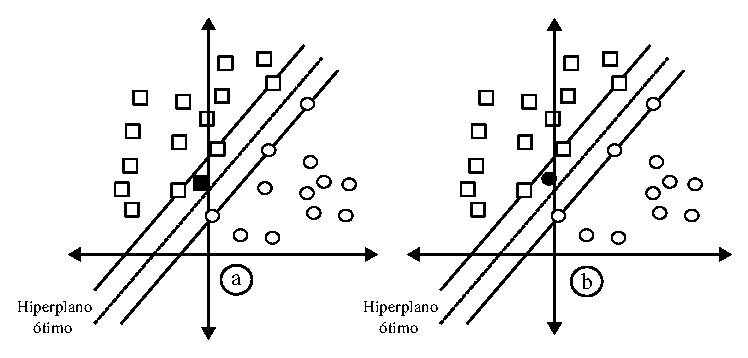
\includegraphics[width=14cm,height=7cm]{./secoes/conceitosFundamentais/pics/img/VetoresDeSuporteSVM_casoNaoSeparavel.eps}
  \label{FIGURA_SVM_Caso_Nao_Separavel}
  \vspace{0.1cm}
  \source{Adaptado de \citeonline{Haykin2007}}
\end{figure}

Dessa forma, o problema pode ser visto como um caso especial do caso linearmente separável, permitindo reformular o primal anterior, ver equação \eqref{EQU_SVM_LAGRANGIANO_PRIMAL}, como
\begin{align}
\nonumber J(\mathbf{w}, b, \alpha, \beta, \xi) &= \frac{1}{2}\mathbf{w}^{T}\mathbf{w} + C\sum\limits_{i=1}^{N} \left( \xi_{i} \right)\\ &- \sum\limits_{i=1}^{N} \left\{\alpha_{i}[d_{i}(\mathbf{w}^{T}\mathbf{x} + b) - 1 + \xi_{i}]\right\} - \sum\limits_{i=1}^{N} \left( \beta_{i} \xi_{i} \right)  \label{EQU_SVM_LAGRANGIANO_PRIMAL_NAO_SEPARAVEL}
\end{align}
cujo ponto de mínimo é dado pelas condições
\begin{align}
 \frac{\partial J(\mathbf{w}, b, \alpha, \beta, \xi)}{\partial \mathbf{w}} = 0	\label{EQU_SVM_PONTO_SELA_W_NAO_SEPARAVEL}\\
 \frac{\partial J(\mathbf{w}, b, \alpha, \beta, \xi)}{\partial b} = 0  			\label{EQU_SVM_PONTO_SELA_B_NAO_SEPARAVEL}\\
 \frac{\partial J(\mathbf{w}, b, \alpha, \beta, \xi)}{\partial \xi} = 0  		\label{EQU_SVM_PONTO_SELA_xi_NAO_SEPARAVEL}
\end{align}
aplicando a condição \eqref{EQU_SVM_PONTO_SELA_W} na equação \eqref{EQU_SVM_LAGRANGIANO_PRIMAL_NAO_SEPARAVEL} obtem-se 
\begin{align}
\mathbf{w} = \sum\limits_{i=1}^{N} \left( \alpha_{i}d_{i}\mathbf{x_{i}} \right)  \label{EQU_SVM_PONTO_SELA_W_RESTRICAO_OBTIDA_NAO_SEPARAVEL}
\end{align}
aplicando a condição \eqref{EQU_SVM_PONTO_SELA_B} na equação \eqref{EQU_SVM_LAGRANGIANO_PRIMAL_NAO_SEPARAVEL} obtem-se 
\begin{align}
\sum\limits_{i=1}^{N} \left( \alpha_{i}d_{i} \right) = 0 \label{EQU_SVM_PONTO_SELA_B_RESTRICAO_OBTIDA_NAO_SEPARAVEL}
\end{align}
aplicando a condição \eqref{EQU_SVM_PONTO_SELA_xi_NAO_SEPARAVEL} na equação \eqref{EQU_SVM_LAGRANGIANO_PRIMAL_NAO_SEPARAVEL} obtem-se
\begin{align}
\alpha_{i}+\beta_{i} = C \label{EQU_SVM_PONTO_SELA_xi_RESTRICAO_OBTIDA_NAO_SEPARAVEL}
\end{align}
segundo \citeonline{LIMA2004} as condições de KKT para o problema são
\begin{align}
\alpha_{i}[d_{i}(w^{T}x + b) - 1 + \xi_{i}] = 0 \label{EQU_SVM_KKT1_NAO_SEPARAVEL}\\
\alpha_{i} \geq 0 \label{EQU_SVM_KKT2_NAO_SEPARAVEL}\\
\beta_{i} \geq 0 \label{EQU_SVM_KKT3_NAO_SEPARAVEL}\\
\beta_{i}\xi_{i} = 0 \label{EQU_SVM_KKT4_NAO_SEPARAVEL}
\end{align}
utilizando as condições \eqref{EQU_SVM_PONTO_SELA_W_RESTRICAO_OBTIDA_NAO_SEPARAVEL} até \eqref{EQU_SVM_KKT4_NAO_SEPARAVEL} é possível escrever o problema dual como
\begin{align}
Q(\alpha) = \sum\limits_{i=1}^{N} \left( \alpha_{i} \right) - \frac{1}{2} \sum\limits_{i=1}^{N} \left( \sum\limits_{j=1}^{N} \left( \alpha_{i}\alpha_{j}d_{i}d_{j}\mathbf{x_{i}}^{T}\mathbf{x_{j}} \right) \right) \label{EQU_SVM_OBJETIVO_NAO_SEPARAVEL_DUAL} 
\end{align}
com as restrições
\begin{align}
\sum\limits_{i=1}^{N} \left( \alpha_{i}d_{i} \right) &= 0 \\
0 < \alpha_{i} &\leq C	\qquad \textrm{ para } i = 1, 2, 3, \ldots, N \label{EQU_RESTRICAO_MARGEM_SUAVE_EXTRA}
\end{align}
a qual é idêntica ao caso separável acrescida de uma condição limitante (equação \eqref{EQU_RESTRICAO_MARGEM_SUAVE_EXTRA}) para o valor dos multiplicadores de Lagrange. O cálculo dos valores ótimos \(\mathbf{w_{0}}\) e \(b_{0}\) é feito de forma análoga ao caso linear acrescida da restrição \eqref{EQU_RESTRICAO_MARGEM_SUAVE_EXTRA}. Determinar o vetor de peso ótimo (\(\mathbf{w_{0}}\)) pode ser feito usando a equação \eqref{EQU_SVM_PONTO_SELA_W_RESTRICAO_OBTIDA_NAO_SEPARAVEL}, tal que
\begin{align}
\mathbf{w_{0}} = \sum\limits_{i=1}^{N_{S}} \left( \alpha_{0,i}d_{i}\mathbf{x_{i}} \right) \label{EQU_SVM_W_OTIMO_MARGEM_SUAVE} 
\end{align}
com a restrição
\begin{align}
\nonumber 0 < \alpha_{i} &\leq C
\end{align}
em que \(N_{S}\) são os vetores de suporte e os valores de \(\alpha\) satisfazem \eqref{EQU_RESTRICAO_MARGEM_SUAVE_EXTRA}. Para o cálculo do bias ótimo (\(b_{0}\)) pode-se utilizar \(\mathbf{w_{0}}\) e 
\begin{align}
g(\mathbf{x^{s}}) = \mathbf{w_{0}^{T}}\mathbf{x^{s}} + b_{0} = \pm 1
\end{align}
e pode-se utilizar a relação \(d_{i}^{2} = 1\) obtendo
\begin{align}
b_{0} &= \frac{\sum\limits_{j = 1}^{N_{S}} \left( d_{j} - \sum\limits_{i=1}^{N_{S}} \left( \alpha_{0,i}d_{i}\mathbf{x_{i}}^{T}\mathbf{x^{s}} \right) \right)}{N_{S}} 
\end{align}
com a restrição
\begin{align}
\nonumber 0 < \alpha_{i} &\leq C
\end{align}
em que \(\mathbf{x^{s}}\) é um vetor de suporte cujo multiplicador de Lagrange é diferente de zero e os valores de \(\alpha\) satisfazem \eqref{EQU_RESTRICAO_MARGEM_SUAVE_EXTRA}.

%KERNEL TRICK
Quando uma fronteira de decisão linear não for adequado, como na figura \ref{FIGURA_SVM_Caso_Nao_Separavel_KERNEL_TRICK}, é possível mapear os dados de entrada para um espaço de dimensão superior, solucionar o problema que potencialmente se torna linear e mapea-lo novamente para um espaço de dimensão original \cite{Haykin2007}.
\begin{figure}[hbt]
  \centering
  \caption{SVM com dados não linearmente separáveis}
  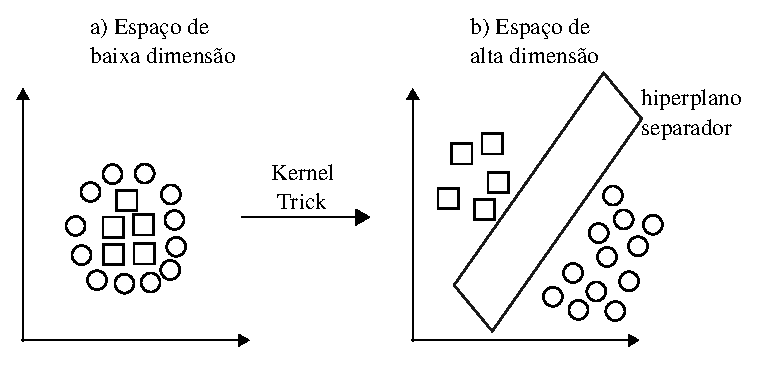
\includegraphics[width=11cm,height=5cm]{./secoes/conceitosFundamentais/pics/img/kernelTrick.eps}
  \label{FIGURA_SVM_Caso_Nao_Separavel_KERNEL_TRICK}
  \source{Adaptado de \citeonline{MachineLearningwithR2013}}
\end{figure}
Para compreender este mapeamento serão alterados alguns detalhes das soluções já apresentadas para os casos anteriores. A equação \eqref{EQU_SVM_W_OTIMO} será reescrita como
\begin{align}
\sum\limits_{i=1}^{N_{S}} \left( \alpha_{i}d_{i}\mathbf{\phi^{T}}(x_{i})\mathbf{\phi}(x) \right) = 0
\end{align}
em que a função \(\mathbf{\phi^{T}}(x_{i})\mathbf{\phi}(x_{i})\) é um produto interno de valores que pode ser definido como
\begin{align}
k(x, x_{i}) = \mathbf{\phi^{T}}(x_{i})\mathbf{\phi}(x) \label{KERNEL_GENERICO}
\end{align}
sendo a equação \eqref{KERNEL_GENERICO} um \emph{Kernel}, o qual é responsável por mapear os dados em alta dimensão \cite{Shawe2004}. Agora é possível reescrever o hiperplano ótimo como
\begin{align}
\sum\limits_{i=1}^{N_{S}} \left( \alpha_{i}d_{i}k(\mathbf{x}, \mathbf{x_{i}}) \right) = 0
\end{align}
com o uso da função de \emph{kernel} \(k\) é desnecessário calcular o vetor de pesos ótimo \(\mathbf{w_{0}}\), este fato é conhecido por \emph{kernel trick}. Por fim, com o uso do \emph{kernel trick} é possível reescrever o problema de otimização dual como
\begin{align}
Q(\alpha) = \sum\limits_{i=1}^{N} \left( \alpha_{i} \right) - \frac{1}{2} \sum\limits_{i=1}^{N} \left( \sum\limits_{j=1}^{N} \left( \alpha_{i}\alpha_{j}d_{i}d_{j} k(\mathbf{x_{i}}, \mathbf{x_{j}}) \right) \right)
\end{align}
com as restrições
\begin{align}
\sum\limits_{i=1}^{N} \left( \alpha_{i}d_{i} \right) &= 0 \\
0 < \alpha_{i} &\leq C	\qquad \textrm{ para } i = 1, 2, 3, \ldots, N
\end{align}
que é idêntico ao caso não separável acrescido da função de \emph{kernel}. Alguns tipos de função \emph{Kernel} utilizadas \cite{Haykin2007, Burges1998} são:
\begin{align}
K(x, y) &= (\mathbf{x}^{T}\mathbf{y} + 1)^{p}											&\textrm{ Polinomial } \\
K(x, y) &= \exp \left( -\frac{1}{2\sigma^{2}}||\mathbf{x} - \mathbf{y}||^{2} \right)  	&\textrm{ Radial }	 \\
K(x, y) &= \tanh(coef0(\mathbf{x}^{T}\mathbf{y}) -  \delta)  							&\textrm{ Sigmoide }	 \\
K(x, y) &= (\mathbf{x}^{T}\mathbf{y})													&\textrm{ Linear } 
\end{align}
sendo \(p, \sigma, \delta\) e \(coef0\) parâmetros passados pelo usuário. A solução deste problema é idêntica para o caso anterior acrescentando a função de \emph{kernel}.

\section{Recomendação por regressão}\label{SEC_RECOMENDACAO_REGRESSAO}
Segundo \citeonline{HanKamber2011} a diferença entre classificar e efetuar uma regressão é que a última tem por objetivo predizer valores contínuos ao invés de discretos.

\subsection{Regressão com SVM}
O SVM para regressão tem por objetivo aproximar ao máximo o hiperplano ótimo dos dados com uma dada tolerância para erros \cite{LIMA2004}. Dado este objetivo, é necessário um modelo insensível em relação a pequenas alterações nos parâmetros. Para atingir este objetivo deve-se utilizar alguma métrica que quantifique a robustez e permita minimizar a degradação máxima do SVM para um determinado valor de insensibilidade denominado \(\epsilon\) \cite{Haykin2007}. Será usada a função
\begin{align}
L_{\epsilon}(d, y) &= 	\begin{cases}\label{EQU_FUNCAO_PERDA_VAPNIK}
							|d - y| - \epsilon  &\textrm{para } |d - y| \geq \epsilon \\
							0					&\textrm{caso contrário}
						\end{cases} \\
y &= \mathbf{w^{T}}\bm{\phi(x)} + b
\end{align}
proposta por \citeonline{Vapnik1988}, em que \(\epsilon\) é definido pelo usuário, \(d\) é o rótulo da instância e \(y\) é a saída do preditor. 
\begin{figure}[hbt]
  \centering
  \caption{Tubo de insensibilidade}
  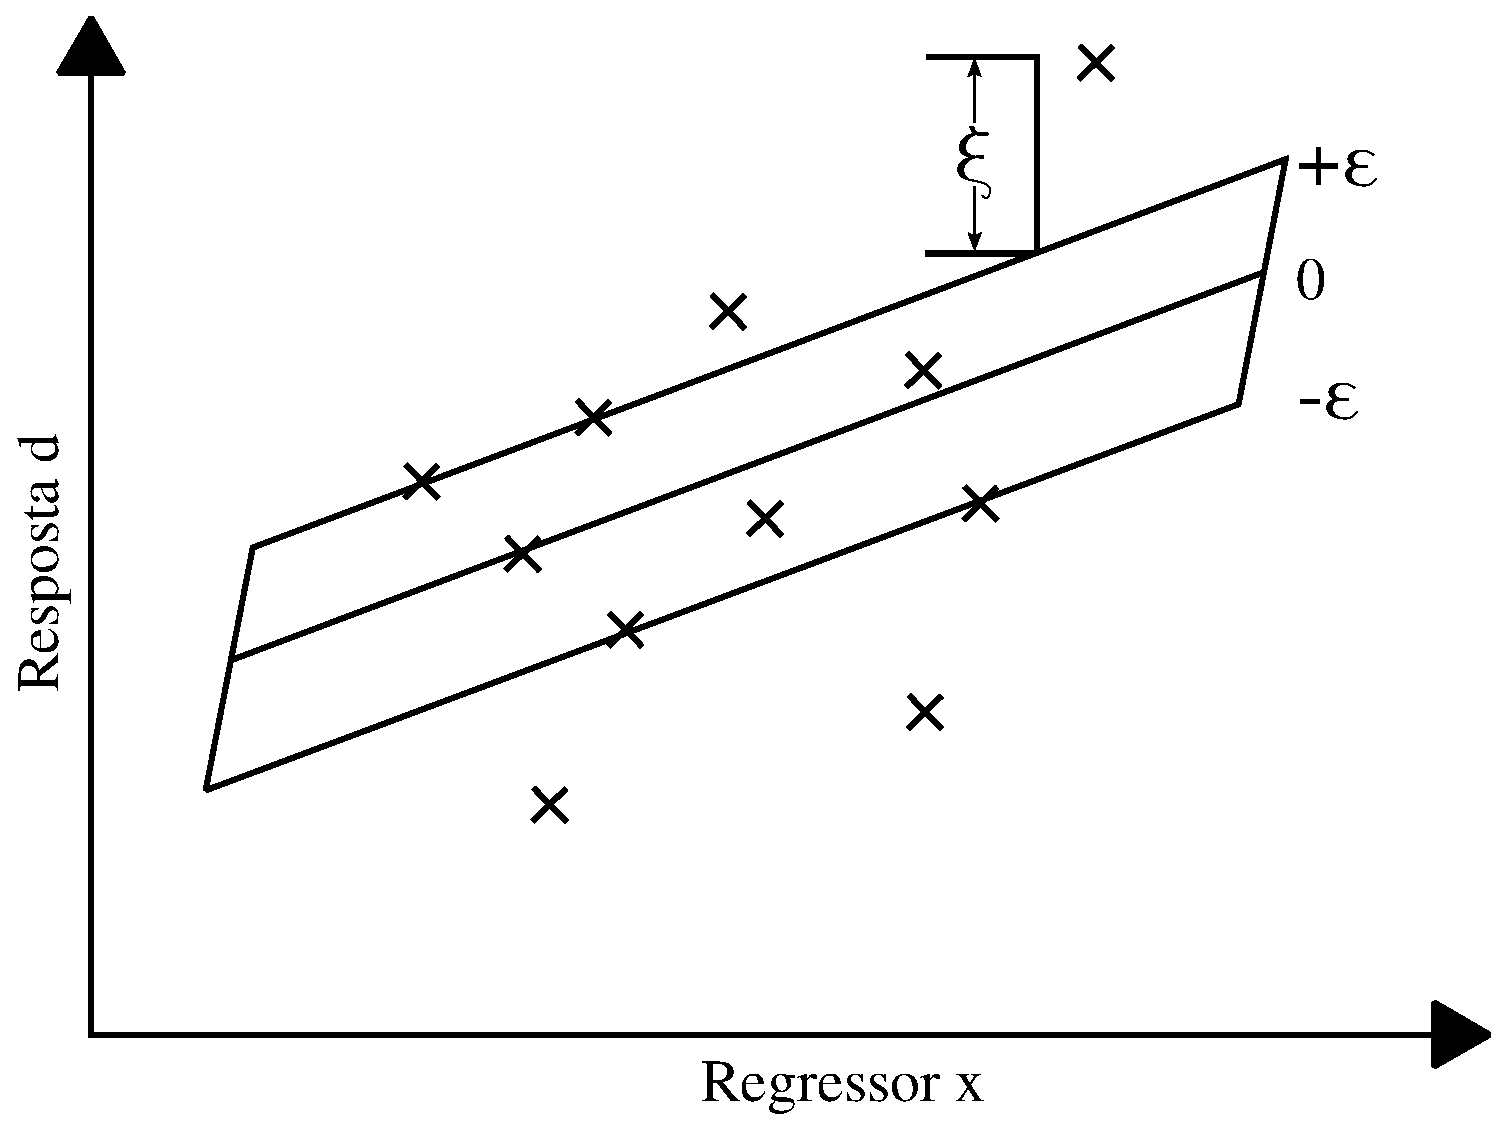
\includegraphics[width=8cm,height=5cm]{./secoes/conceitosFundamentais/pics/img/tuboRobustez.eps}
  \label{FIGURA_SVM_TUBO_INSENSIBILIDADE}
  \source{Adaptado de \citeonline{Haykin2007}}
\end{figure}

A figura \ref{FIGURA_SVM_TUBO_INSENSIBILIDADE} apresenta graficamente a relação entre a função de perda \eqref{EQU_FUNCAO_PERDA_VAPNIK} e o regressor, deve-se ressaltar que o valor de erro só será contabilizado se o valor do erro \(\xi\) satisfizer a seguinte inequação \(|d - y| \geq \epsilon\).
\begin{figure}[hbt]
  \centering
  \caption{Gráfico da função perda}
  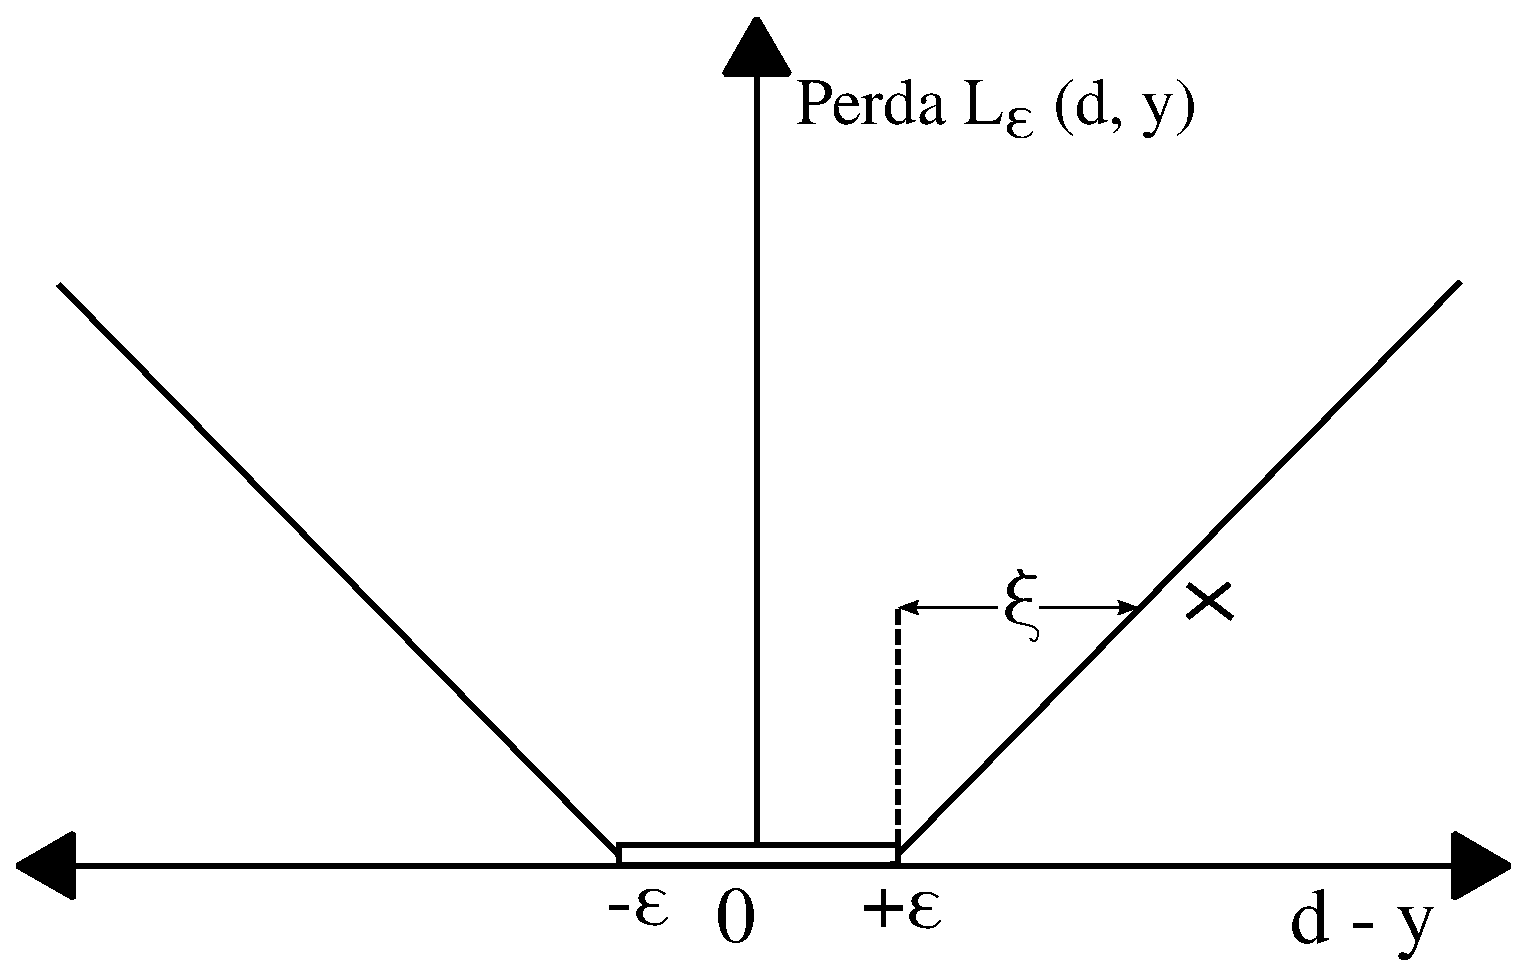
\includegraphics[width=9cm,height=6cm]{./secoes/conceitosFundamentais/pics/img/tuboRobustezComFolga.eps}
  \label{FIGURA_SVM_GRAFICO_FUNCAO_PERDA}
  \source{Adaptado de \citeonline{Haykin2007}}
\end{figure}

A figura \ref{FIGURA_SVM_GRAFICO_FUNCAO_PERDA} exibe a função de perda \ref{EQU_FUNCAO_PERDA_VAPNIK} em função do erro. Dessa forma, fica claro que o valor de \(\epsilon\) é considerado um limiar, a partir do qual o erro começa a ser calculado. Adaptar o SVM para regressão significa encontrar duas variáveis, \(\mathbf{w}\) e \(b\), para a relação de regressão definida por
\begin{align}
d = \mathbf{w}^{T}\mathbf{x} + b
\end{align}
em que \(d\) é a variável resposta e \(\mathbf{x}\) são as variáveis preditoras. A função perda \eqref{EQU_FUNCAO_PERDA_VAPNIK} permite adaptar o problema de otimização formulado como \eqref{EQU_SVM_MARGEM_EQUIVALENTE_MAXIMIZAR} na seção \ref{SEC_CONCEITOS_FUNDAMENTAIS_SVM_CLASSIFICACAO} para
\begin{align}
\Phi(w) =  \frac{1}{2}||\mathbf{w^{T}}\mathbf{w}|| + C \sum\limits_{i=1}^{N} L_{\epsilon}(d, y) \label{EQU_SVM_REGRESSAO_MINIMIZAR}
\end{align}
com as seguintes restrições
\begin{align}
d_{i} - y_{i} &\leq \epsilon + \xi					 \label{EQU_SVM_REGRESSAO_RESTRICAO01} 		\\
y_{i} - d  &\leq \epsilon + \xi^{'}			 \label{EQU_SVM_REGRESSAO_RESTRICAO02} 		\\
\xi^{'}, \xi &\geq 0 \qquad \textrm{ para } i =1, 2, 3 \ldots N \label{EQU_SVM_REGRESSAO_RESTRICAO03}
\end{align}
nas quais \(\xi\) e \(\xi^{'}\) são variáveis de folga, positivas e idênticas a definida no caso não separável do classificador (ver seção \ref{SEC_CONCEITOS_FUNDAMENTAIS_SVM_CLASSIFICACAO}). Utilizando as restrições \eqref{EQU_SVM_REGRESSAO_RESTRICAO01}, \eqref{EQU_SVM_REGRESSAO_RESTRICAO02} e \eqref{EQU_SVM_REGRESSAO_RESTRICAO03} e a função objetivo \eqref{EQU_SVM_REGRESSAO_MINIMIZAR} é possível construir o Lagrangiano Primal, como no caso da formulação do SVM para classificação (ver seção \ref{SEC_CONCEITOS_FUNDAMENTAIS_SVM_CLASSIFICACAO}), obtendo
\begin{align}
\nonumber J(\mathbf{w}, \xi^{'}, \xi, \alpha, \alpha^{'}, \gamma, \gamma^{'}) = \frac{1}{2}||\mathbf{w}^{T}\mathbf{w}|| + C \sum\limits_{i=1}^{N} \xi_{i} + \xi_{i}^{'} - \sum\limits_{i=1}^{N} ( \gamma\xi_{i} + \gamma^{'}\xi_{i}^{'} ) \\
-\sum\limits_{i=1}^{N}\alpha_{i}((\mathbf{w^{T}x}) + b - d_{i}+ \epsilon + \xi_{i}) - \sum\limits_{i=1}^{N}\alpha_{i}^{'}(d_{i} - (\mathbf{w^{T}x}) - b + \epsilon + \xi_{i}^{'}) \label{EQU_SVM_REGRESSAO_LAGRANGIANO_PRIMAL}
\end{align}
a solução do Lagrangiano \eqref{EQU_SVM_REGRESSAO_LAGRANGIANO_PRIMAL} é dada no ponto de sela (análoga ao caso não separável do classificador na seção \ref{SEC_CONCEITOS_FUNDAMENTAIS_SVM_CLASSIFICACAO}). Dessa forma, deve-se calcular suas derivadas parciais em relação a \(\mathbf{w}\), \(b\), \(\xi\) e \(\xi^{'}\) e igualar todas a zero \cite{Haykin2007} obtendo as restrições
\begin{align}
\frac{\partial J(\mathbf{w}, \xi^{'}, \xi, \alpha, \alpha^{'}, \gamma, \gamma^{'})}{\partial \mathbf{w}} = 0	\label{EQU_SVM_REGRESSAO_PONTO_SELA_W}\\
\frac{\partial J(\mathbf{w}, \xi^{'}, \xi, \alpha, \alpha^{'}, \gamma, \gamma^{'})}{\partial b} = 0  	\label{EQU_SVM_REGRESSAO_PONTO_SELA_B}\\
\frac{\partial J(\mathbf{w}, \xi^{'}, \xi, \alpha, \alpha^{'}, \gamma, \gamma^{'})}{\partial \xi} = 0	\label{EQU_SVM_REGRESSAO_PONTO_SELA_XI}\\
\frac{\partial J(\mathbf{w}, \xi^{'}, \xi, \alpha, \alpha^{'}, \gamma, \gamma^{'})}{\partial \xi^{'}} = 0  	\label{EQU_SVM_REGRESSAO_PONTO_SELA_XI_LINHA}
\end{align}
aplicando a condição \eqref{EQU_SVM_REGRESSAO_PONTO_SELA_W} na equação \eqref{EQU_SVM_REGRESSAO_LAGRANGIANO_PRIMAL} obtem-se 
\begin{align}
\mathbf{\hat{w}} = \sum\limits_{i=1}^{N} (\alpha_{i} - \alpha^{'}_{i})x \label{EQU_SVM_REGRESSAO_PESO_W}
\end{align}
aplicando a condição \eqref{EQU_SVM_REGRESSAO_PONTO_SELA_B} na equação \eqref{EQU_SVM_REGRESSAO_LAGRANGIANO_PRIMAL} obtem-se 
\begin{align}
\sum\limits_{i=1}^{N} (\alpha_{i} - \alpha^{'}_{i}) = 0
\end{align}
aplicando a condição \eqref{EQU_SVM_REGRESSAO_PONTO_SELA_XI} na equação \eqref{EQU_SVM_REGRESSAO_LAGRANGIANO_PRIMAL} obtem-se 
\begin{align}
\alpha + \gamma = C
\end{align}
aplicando a condição \eqref{EQU_SVM_REGRESSAO_PONTO_SELA_XI_LINHA} na equação \eqref{EQU_SVM_REGRESSAO_LAGRANGIANO_PRIMAL} obtem-se 
\begin{align}
\alpha^{'} + \gamma^{'} = C
\end{align}
\noindent
o parâmetro desejado \(\mathbf{\hat{w}}\) foi obtido pela equação \eqref{EQU_SVM_REGRESSAO_PESO_W} em função dos multplicadores de Lagrange \(\alpha^{'}, \alpha\). O valor de \(\hat{b}\) pode ser obtido pelas condições de KKT, que segundo \citeonline{Haykin2007}, são
\begin{align}
\alpha(\epsilon + \xi + d_{i} - y_{i}) &= 0 \label{EQU_SVM_REGRESSAO_KKT1}\\
\alpha^{'}(\epsilon + \xi^{'} - d_{i} + y_{i}) &= 0 \label{EQU_SVM_REGRESSAO_KKT2}\\
(C-\alpha)\xi &= 0 \label{EQU_SVM_REGRESSAO_KKT3}\\
(C-\alpha^{'})\xi^{'} &= 0 \label{EQU_SVM_REGRESSAO_KKT4}
\end{align}
analisando as equações \eqref{EQU_SVM_REGRESSAO_KKT1} e \eqref{EQU_SVM_REGRESSAO_KKT2} pode-se concluir que instâncias nas quais \(C=\alpha\) ou \(C=\alpha^{'}\) residem fora das variáveis de folga \(\xi\) e \(\xi^{'}\). Multiplicando \eqref{EQU_SVM_REGRESSAO_KKT1} por \(\alpha\) e \eqref{EQU_SVM_REGRESSAO_KKT2} por \(\alpha^{'}\) e somando-as obtem-se
\begin{align}
\alpha\alpha^{'}(2\epsilon + \xi + \xi^{'})=0
\end{align}
sempre que \(\epsilon > 0\), \(\xi > 0\) e \(\xi^{'} > 0\) implica que \(\alpha\alpha^{'} = 0\), logo ambos os multiplicadores de Lagrange não podem ser zero simultaneamente. Pelas equações \eqref{EQU_SVM_REGRESSAO_KKT3} e \eqref{EQU_SVM_REGRESSAO_KKT4} pode-se escrever
\begin{align}
\xi  &= 0		\qquad \textrm{ para } 0 < \alpha < C		\label{EQU_SVM_REGRESSAO_CONDICAO1}\\
\xi^{'} &= 0	\qquad \textrm{ para }  0 < \alpha^{'} < C	\label{EQU_SVM_REGRESSAO_CONDICAO2}
\end{align}
as equações \eqref{EQU_SVM_REGRESSAO_CONDICAO1} e \eqref{EQU_SVM_REGRESSAO_CONDICAO2} usadas em \eqref{EQU_SVM_REGRESSAO_KKT1} e \eqref{EQU_SVM_REGRESSAO_KKT2} implicam que  
\begin{align}
\epsilon  - d_{i} + y_{i} &= 0	\qquad \textrm{ para } 0 < \alpha < C		\label{EQU_SVM_REGRESSAO_CONDICAO3}\\
\epsilon  + d_{i} - y_{i} &= 0	\qquad \textrm{ para }  0 < \alpha^{'} < C	\label{EQU_SVM_REGRESSAO_CONDICAO4}
\end{align}
agora que as condições de KKT e suas implicações foram discutidas para concluir o cálculo do estimador ótimo da função de regressão 
dado por 
\begin{align}
y = \mathbf{\hat{w}^{T}x} + \hat{b} \label{EQU_SVM_REGRESSAO_ESTIMADOR_OTIMO}
\end{align}
sendo que \(\mathbf{\hat{w}}\) já foi calculado pela equação \eqref{EQU_SVM_REGRESSAO_PESO_W}. Falta calcular \(\hat{b}\) que será calculado por meio da equação \eqref{EQU_SVM_REGRESSAO_ESTIMADOR_OTIMO} e restrito às condições \eqref{EQU_SVM_REGRESSAO_CONDICAO3} e \eqref{EQU_SVM_REGRESSAO_CONDICAO4} obtendo
\begin{align}
\hat{b} = d_{i} - \mathbf{\hat{w}^{T}x} -\epsilon	\qquad \textrm{ para } 0 < \alpha < C		\label{EQU_SVM_REGRESSAO_CONDICAO6}\\
\hat{b} = d_{i} - \mathbf{\hat{w}^{T}x} +\epsilon	\qquad \textrm{ para }  0 < \alpha^{'} < C	\label{EQU_SVM_REGRESSAO_CONDICAO7}
\end{align}
Com o valor de \(\hat{w}\) obtido da equação \eqref{EQU_SVM_REGRESSAO_PESO_W} e dados \(\epsilon\) e \(d_{i}\) foi possível computar \(\hat{b}\). Dessa forma o estimador ótimo \eqref{EQU_SVM_REGRESSAO_ESTIMADOR_OTIMO} pode ser usado para predizer valores.

\subsection{MARS}
O algoritmo \emph{Multivariate Adaptive Regression Splines} (MARS), segundo \citeonline{StatisticalLearning2001}, é uma generalização da regressão linear por função degrau. Para tal, usa-se segmentos lineares de funções com a seguinte estrutura
\begin{align}
(x-t)_{+} &= \begin{cases}
x-t, \textrm{ se } x > t \\
0,   \textrm{ caso contrário}
\end{cases}
\\
(t-x)_{+} &= \begin{cases}
t-x, \textrm{ se } x < t \\
0, \textrm{ caso contrário}
\end{cases} 
\end{align}

Assim como na figura \ref{FIGURA_MARS_FUNCAO_ESPELHO}, na qual são visualizadas as funções espelho \((x-0.5)_{+}\) e \((0.5-x)_{+}\), cada segmento é representado por uma função linear e possui um nó no valor de \(x\). Diversas funções espelho são unidas para formar o modelo de regressão MARS, que nesse ponto está pronto para predizer valores.

\begin{figure}[hbt]
	\centering
 	  \caption{Funções espelho usadas pelo MARS}
		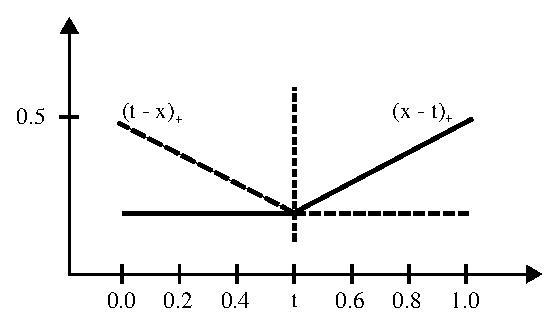
\includegraphics[width=9cm,height=5cm]{./secoes/conceitosFundamentais/pics/img/FuncaoEspelhoMARS.eps}
	\label{FIGURA_MARS_FUNCAO_ESPELHO}
  \source{Adaptado de \citeonline{StatisticalLearning2001}}
\end{figure}

\subsection{Regressão Logística}
A regressão logística prediz valores (variável de resposta) contínuos baseados em valores categóricos ou numéricos contínuos (variáveis preditoras). Sua modelagem ocorre por meio do \emph{generalized linear model} que é uma abordagem unificada para modelar alguns tipos de variáveis \cite{Agresti2015}. Este tipo de modelo é composto por três componentes necessários \cite{Agresti2015, Olsson2002} para predizer valores: i) a distribuição das variáveis; ii) uma função \emph{link}, cujo objetivo é relacionar a média condicional da distribuição com o preditor linear; e iii) o preditor linear. O preditor linear é dado por
\begin{align}
g(\mu_{Y}) = \beta_{0} + \sum\limits_{j = 1}^{P} \beta_{j}X_{j} \label{EQU_PREDITOR_LINEAR}
\end{align}
, a função \emph{link} é dada por
\begin{align}
g(\mu_{Y}) = \log_{e} \left( \frac{ \pi }{ 1 - \pi } \right)	\label{EQU_FUNCAO_LINK}
\end{align}
e a distribuição de probabilidade assumida pela regressão logística é a \emph{binomial}. Em relação às equações \eqref{EQU_PREDITOR_LINEAR} e \eqref{EQU_FUNCAO_LINK} tem-se que \(\pi = \mu_{Y}\) é a média condicional, que significa que a probabilidade de \(Y = 1\), dado um conjunto de valores de \(X\); e \(\frac{\pi}{1 - \pi}\) é a probabilidade de que \(Y = 1\) \cite{Olsson2002}. Usando essas equações e assumindo uma distribuição binomial para os dados, a regressão logística está pronta para predizer valores pois os valores dos coeficientes \(\beta\) foram estimados por maima verossimilhança e substituídos na equação \eqref{EQU_PREDITOR_LINEAR} que agora receberá valores de \(x\) históricos para prever novos valores.

\section{Classificadores compostos}\label{ENSEMBLES} %subsection
Nessa seção serão descritos dois classificadores compostos, denominados dessa forma pois utilizam o resultado de outros classificadores/regressores e o rótulo das instâncias para aprender. O primeiro consiste no uso do classificador SVM (descrito na seção \ref{SEC_CONCEITOS_FUNDAMENTAIS_SVM_CLASSIFICACAO}) sobre o resultado dos outros \(5\) classificadores e \(5\) regressores.
O segundo é um \emph{ensemble} de classificadores conhecido como \emph{Rotation Forest}, o qual foi proposto por \citeonline{Rodriguez2006}.

Ambas as técnicas usam uma matriz \(M\) de entrada, criada pelos autores e apresentada pela tabela~\ref{tabela_matriz_de_dados_classificador_composto}, que contém \(8.614\) casos de recomendação (que são as linhas da tabela) e uma coluna de rótulo. Cada célula da matriz \(M\) representa a posição em que o item removido \(i\) foi recomendado pelo sistema \(j\).
\begin{table}[!htb]
	\tiny
	\centering
	\caption{Matriz de entrada para classificadores compostos}
	\begin{tabular}{|c|c|c|c|c|c|c|c|}  \hline
	
\textbf{$\mathbf{\#}$} & \textbf{Workflow} & \textbf{Sist. $\mathbf{01}$}  & \textbf{$\ldots$}  & \textbf{Sist. $\mathbf{N}$} & \textbf{Ativ. removidas} & \textbf{Rótulo} \\ \hline

1			& 01		  & 12 		   &\(\ldots\) & 1 		   & Ativ $01$ 	& T			\\ \hline
2			& 01 		  & 13 		   &\(\ldots\) & 1         & Ativ $01$ 	& T			\\ \hline
\(\vdots\)  &\(\vdots\)   &\(\vdots\)  &\(\vdots\) &\(\vdots\) &\(\vdots\)  &\(\vdots\) \\ \hline
59			& 01 		  & 1 		   &\(\ldots\) & 1         & Ativ $01$ 	& T			\\ \hline
1			& 01		  & 4 		   &\(\ldots\) & 1         & Ativ $02$	& F			\\ \hline
2			& 01 		  & 7  		   &\(\ldots\) & 1         & Ativ $03$	& F			\\ \hline
\(\vdots\)  &\(\vdots\)   &\(\vdots\)  &\(\vdots\) &\(\vdots\) &\(\vdots\)  &\(\vdots\) \\ \hline
59			& 01 		  & 8          &\(\ldots\) & 2         & Ativ $59$ 	& F 		\\ \hline
			&\(\vdots\)   & 		   & 		   & 		   & 			& 			\\ \hline
1			& 73		  & 9 		   &\(\ldots\) & 10        & Ativ $02$ 	& T			\\ \hline
2			& 73 		  & 18 		   &\(\ldots\) & 0         & Ativ $02$ 	& T			\\ \hline
\(\vdots\)  &\(\vdots\)   &\(\vdots\)  &\(\vdots\) &\(\vdots\) &\(\vdots\)  &\(\vdots\) \\ \hline
59			& 73 		  & 65		   &\(\ldots\) & 6         & Ativ $02$ 	& T			\\ \hline
1			& 73		  & 67 		   &\(\ldots\) & 7         & Ativ $03$ 	& F			\\ \hline
2			& 73 		  & 5 		   &\(\ldots\) & 8 		   & Ativ $04$ 	& F			\\ \hline
\(\vdots\)  &\(\vdots\)   &\(\vdots\)  &\(\vdots\) &\(\vdots\) &\(\vdots\)	&\(\vdots\) \\ \hline
59			& 73          & 14 	       &\(\ldots\) & 9 		   & Ativ $59$ 	& F			\\ \hline
		\end{tabular}
	\label{tabela_matriz_de_dados_classificador_composto}
	\vspace{0.1cm}
	\source{\varAutorData}
\end{table}


%Fica muito feio sem esse newpage, favor não remover :)
%\newpage
\subsection{Análise de Componentes Principais}\label{SUBSECTION_PCA}
A Análise de Componentes Principais (PCA) tem por objetivo maximizar a variância. A abordagem utilizada neste trabalho é  baseada em matriz de covariância. O objetivo da PCA é reduzir dimensões de $p$ para $d$ onde $p < d$.

O algoritmo transforma o conjunto de dados originais por meio de uma combinação linear das variáveis. Os dados são projetados de forma ortogonal. Um exemplo dessa projeção pode ser visualizado na figura \ref{figura01_Projecao_PCA}, extraída de \citeonline{Martinez2004}.
\begin{figure}[!htp]
	\centering
	\caption{Projeção ortogonal dos dados do algoritmo PCA}
	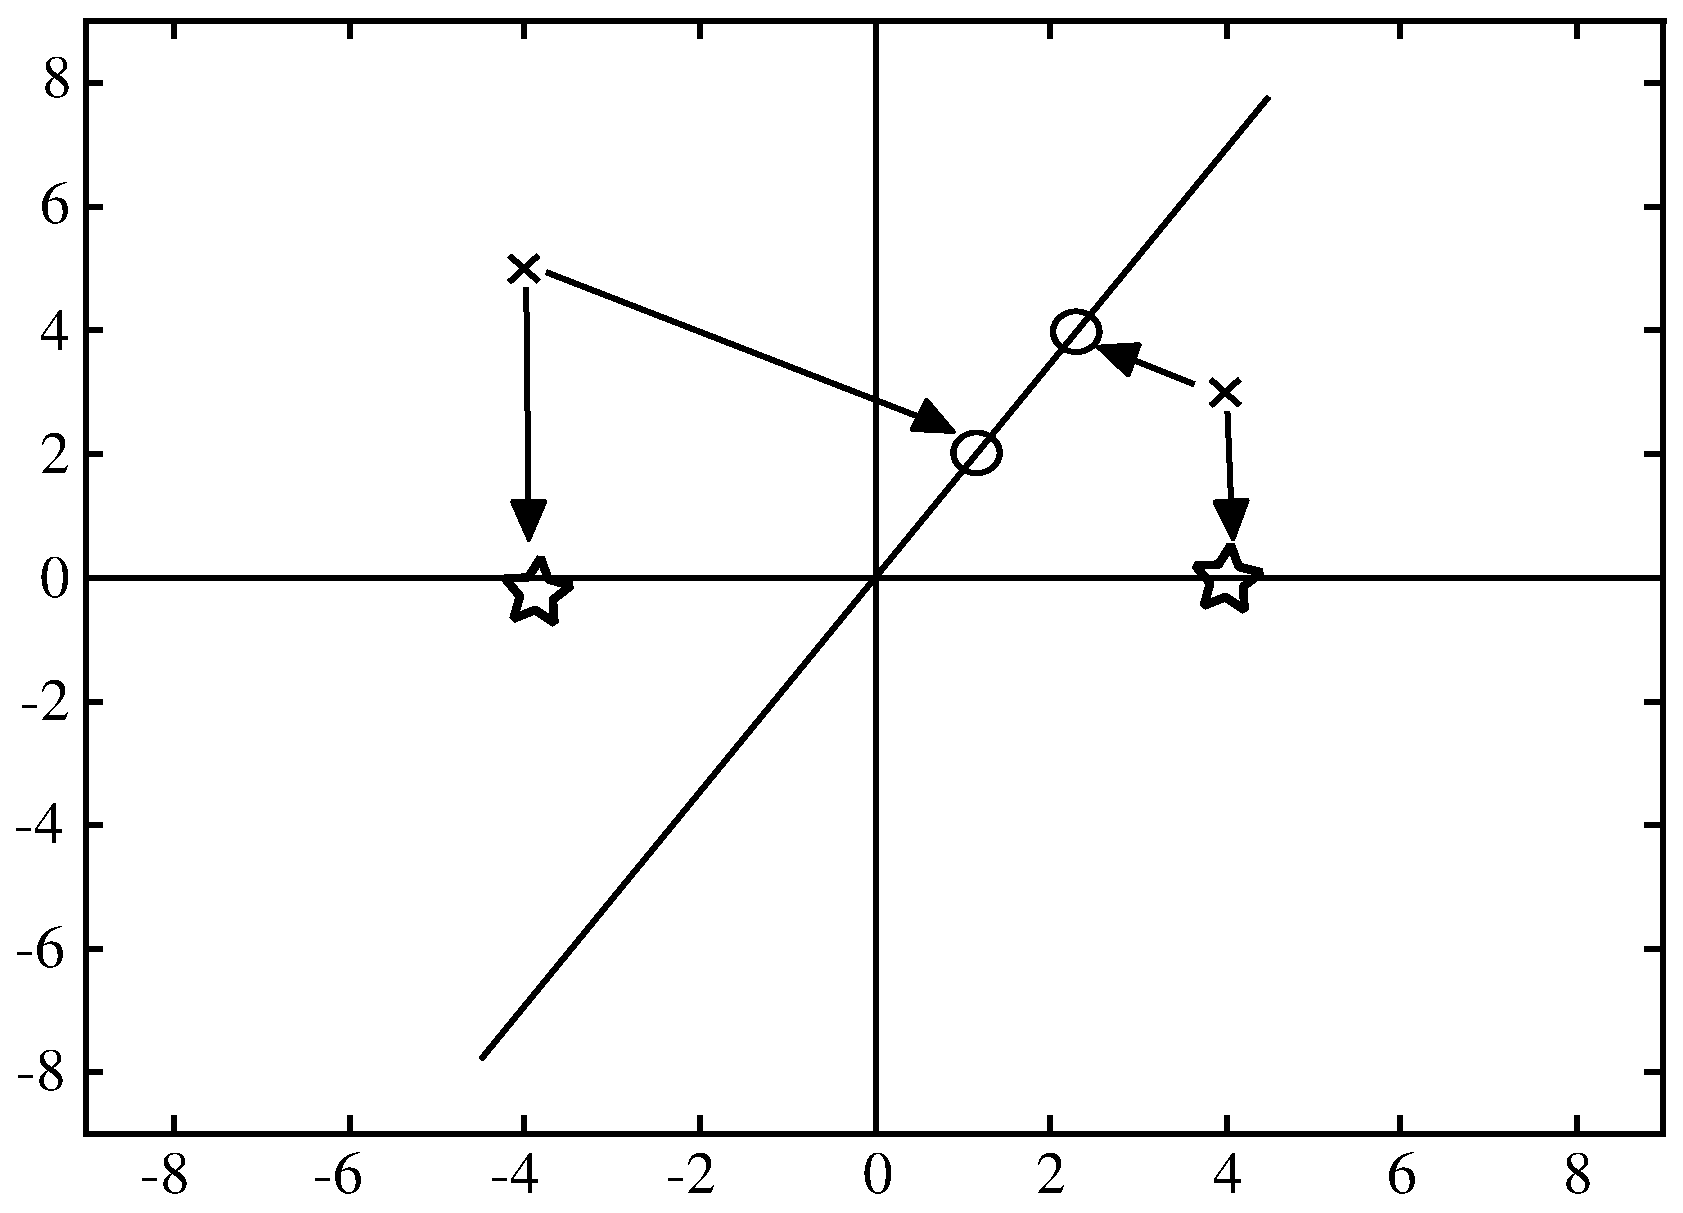
\includegraphics[height=8cm,width=12cm]{./secoes/conceitosFundamentais/pics/img/figura01_Projecao_PCA.eps}
	\vspace{0.1cm}
	\source{Adaptado de \citeonline{Martinez2004}}
	\label{figura01_Projecao_PCA}
\end{figure}

Há duas possíveis implementações de PCA mais usuais, por matriz de correlação e por matriz de covariância. No algoritmo \emph{Rotation Forest} é usada a abordagem de matriz de covariância. O primeiro passo é calcular a matriz de covariância da média dos dados de entrada centralizados, formando uma nova matriz \(N\). Em seguida, são calculados os autovalores e autovetores da matriz \(N\). Por fim, os autovetores são usados para projetar os dados em outro eixo como na figura \ref{figura01_Projecao_PCA}.

\subsection{Rotation Forest}
Um \emph{ensemble} de classificadores é um conjunto de classificadores, com alguma forma de diversificação, que resolvem o mesmo problema (particionado) e juntam suas soluções para chegar em um resultado final. A figura \ref{FIGURA_ENSEMBLE_DE_CLASSIFICADORES} exibe uma arquitetura típica de um \emph{ensemble} de classificadores, na qual o retângulo, sem numeração, representa o conjunto dos dados originais, os retângulos com numeração são as partições, os triângulos são os classificadores e a estrela de sete pontas a união das respostas dos classificadores.
\begin{figure}[hbt]
  \centering
  \caption{Arquitetura de \emph{ensemble} de classificadores}
  	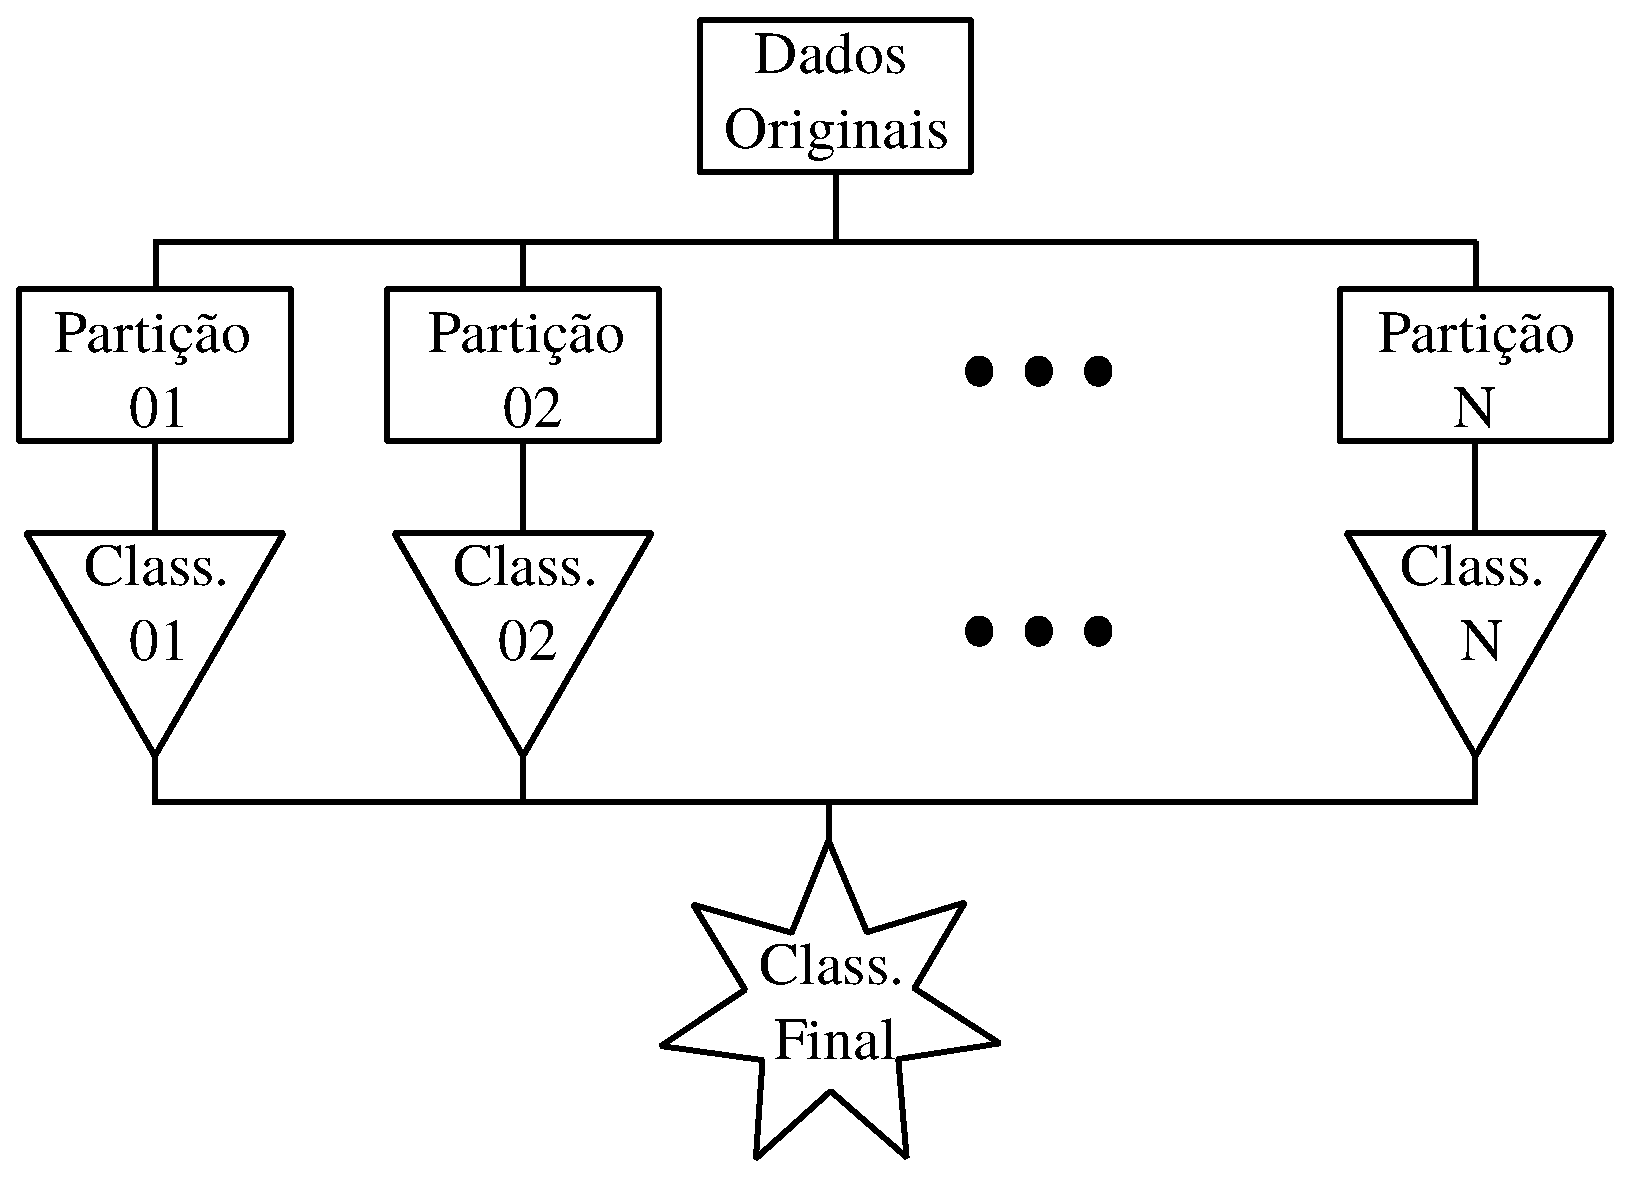
\includegraphics[width=8cm,height=6cm]{./secoes/conceitosFundamentais/pics/img/Ensemble.eps}
  \label{FIGURA_ENSEMBLE_DE_CLASSIFICADORES}
  \vspace{0.1cm}
  \source{Adaptado de \citeonline{Rodriguez2006}}
\end{figure}

A técnica proposta por \citeonline{Rodriguez2006} cria um \emph{ensemble} de classificadores por meio de extração de características. O conjunto de dados é dividido em \(K\) subconjuntos (que é um parâmetro do algoritmo). Em seguida a técnica Principal Component Analysis (PCA) (ver seção \ref{SUBSECTION_PCA}) é aplicada em cada subconjunto. São mantidas todas as componentes principais, o que, segundo os autores, preserva a variabilidade dos dados. O próximo passo é multiplicar o conjunto de características originais pelos componentes principais.  Cada subconjunto é apresentado a seu respectivo classificador, e após cada um destes solucionarem o problema, a instância a ser classificada será atribuída à classe com maior probabilidade. Este valor é obtido pela média de todos os classificadores do \emph{ensemble}.

Considerando que \(x = [x_{i}, \ldots x_{n}]\) é uma instância com \(n\) dimensões, \(X\) é uma matriz de instâncias com dimensões \(N \times n\), \(Y\) é o vetor de rótulos de \(X\), que assumem os valores \(y_{i} = [C_{1}, C_{2}, \ldots, C_{n}]\), seja \(D_{1}, D_{2}, \ldots, D_{L}\) o conjunto de classificadores usados e \(F\) o conjunto de características. Os classificadores usados nesse \emph{ensemble} são todos árvores de classificação e regressão (CART), descritos na seção \ref{SUBSECTION_CART}. A construção do conjunto de treinamento para o classificador \(D_{i}\) pode ser realizado em quatro passos.

Primeiramente o conjunto de dados original é dividido em \(K\) partições disjuntas, seja \(F_{i,j}\) o conjunto das características da partição do classificador \(D_{i}\) e seja \(X_{i,j}\) o conjunto de dados formado pelas características \(F_{i,j}\). Em seguida, para cada classificador, deve-se remover um subconjunto de classes de \(X_{i,j}\) e selecionar uma amostra do tipo \emph{bootstrap} (com reamostragem), com tamanho de \(75\%\) do número de seus objetos. O novo conjunto será denominado \(X_{i,j}^{'}\). O próximo passo é aplicar a PCA em \(X_{i,j}^{'}\) para obter a seguinte matriz de coeficientes
\begin{align}
R_{i} =
\begin{bmatrix}
    a_{i,1}^{(1)}, a_{i,1}^{(2)}, \dots a_{i,1}^{(M_{1})} & [0] 												  & \dots  & [0] \\
    [0] 												  & a_{i,2}^{(1)}, a_{i,2}^{(2)}, \dots a_{i,2}^{(M_{2})} & \dots  & [0] \\
    \vdots 												  & \vdots 												  & \ddots & \vdots \\
    [0] 												  & [0] & \dots  & a_{i,K}^{(1)}, a_{i,K}^{(2)}, \dots a_{i,K}^{(M_{K})}
\end{bmatrix}
\end{align}

Em seguida deve-se rearranjar a matriz \(R_{i}\) para que a ordem dos coeficientes seja a mesma das características de \(F\) criando a matriz \(R_{i}^{a}\). Dessa forma, o classificador \(D_{i}\) pode ser treinado usando \((XR_{i}^{a}, Y)\) como conjunto de treinamento. Para a fase de classificação é usada a seguinte equação
\begin{align}
\mu_{j}(x) = \frac{1}{L}\sum\limits_{i=1}^{L} d_{i,j}(XR_{i}^{a})  \qquad j = 1, \ldots, c \label{EQU_FUNCAO_DISCRIMINANTE_ROTATIONFOREST}
\end{align}
na qual \(d_{i,j}(XR_{i}^{a})\) é a probabilidade atribuída pelo classificador \(D_{i}\) que \(x\) seja da classe \(C_{j}\), \(c\) é o número total de classes do problema e a equação \eqref{EQU_FUNCAO_DISCRIMINANTE_ROTATIONFOREST} representa a confiança média de todos os classificadores do conjunto \(D\) de que \(x\) seja da classe \(C_{j}\).
